\documentclass[letterpaper,12pt]{article}

\usepackage{threeparttable}
\usepackage{geometry}
\geometry{letterpaper,tmargin=1in,bmargin=1in,lmargin=1.25in,rmargin=1.25in}
\usepackage[format=hang,font=normalsize,labelfont=bf]{caption}
\usepackage{amsmath}
\usepackage{multirow}
\usepackage{array}
\usepackage{delarray}
\usepackage{amssymb}
\usepackage{amsthm}
\usepackage{lscape}
\usepackage{natbib}
\usepackage{setspace}
\usepackage{float,color}
\usepackage[pdftex]{graphicx}
\usepackage{pdfsync}
\usepackage{verbatim}
\synctex=1
\usepackage{hyperref}
\hypersetup{colorlinks,linkcolor=red,urlcolor=blue,citecolor=red}
\usepackage{bm}
\theoremstyle{definition}
\newtheorem{theorem}{Theorem}
\newtheorem{acknowledgement}[theorem]{Acknowledgement}
\newtheorem{algorithm}[theorem]{Algorithm}
\newtheorem{axiom}[theorem]{Axiom}
\newtheorem{case}[theorem]{Case}
\newtheorem{claim}[theorem]{Claim}
\newtheorem{conclusion}[theorem]{Conclusion}
\newtheorem{condition}[theorem]{Condition}
\newtheorem{conjecture}[theorem]{Conjecture}
\newtheorem{corollary}[theorem]{Corollary}
\newtheorem{criterion}[theorem]{Criterion}
\newtheorem{definition}{Definition} % Number definitions on their own
\newtheorem{derivation}{Derivation} % Number derivations on their own
\newtheorem{example}[theorem]{Example}
\newtheorem{exercise}[theorem]{Exercise}
\newtheorem{lemma}[theorem]{Lemma}
\newtheorem{notation}[theorem]{Notation}
\newtheorem{problem}[theorem]{Problem}
\newtheorem{proposition}{Proposition} % Number propositions on their own
\newtheorem{remark}[theorem]{Remark}
\newtheorem{solution}[theorem]{Solution}
\newtheorem{summary}[theorem]{Summary}
\bibliographystyle{aer}
\newcommand\ve{\varepsilon}
\renewcommand\theenumi{\roman{enumi}}
\newcommand\norm[1]{\left\lVert#1\right\rVert}

\begin{document}

\begin{titlepage}
\title{An Open Source Macroeconomic Model \\
       for Dynamic Scoring of Tax Policy
       \thanks{
       Put thanks here.}
       }
\author{
  Jason DeBacker\footnote{Middle Tennessee State University, Department of Economics and Finance, BAS N306, Murfreesboro, TN 37132, (615) 898-2528,\href{mailto:jason.debacker@mtsu.edu}{jason.debacker@mtsu.edu}.} \\[-2pt]
  \and
  Richard W. Evans\footnote{Brigham Young University, Department of Economics, 167 FOB, Provo, Utah 84602, (801) 422-8303, \href{mailto:revans@byu.edu}{revans@byu.edu}.} \\[-2pt]
  \and
  Evan Magnusson\footnote{Brigham Young University, Department of Economics, 163 FOB, Provo, Utah 84602, \href{mailto:evanmag42@gmail.com}{evanmag42@gmail.com}.} \\[-2pt]
  \and
  Kerk L. Phillips\footnote{Brigham Young University, Department of Economics, 166 FOB, Provo, Utah 84602, (801) 422-5928, \href{mailto:kerk_phillips@byu.edu}{kerk\_phillips@byu.edu}.} \\[-2pt]
  \and
  Isaac Swift\footnote{Brigham Young University, Department of Economics, 163 FOB, Provo, Utah 84602, \href{mailto:isaacdswift@gmail.com}{isaacdswift@gmail.com}.} \\[-2pt]}
\date{August 2014 \\
  \scriptsize{(version 14.08.c)}}
\maketitle
\begin{abstract}
\normalsize{Put abstract here.

\vspace{3mm}

\noindent\textit{keywords:}\: Put keywords here.

\vspace{3mm}

\noindent\textit{JEL classification:} Put JEL codes here.}
\end{abstract}
\thispagestyle{empty}
\end{titlepage}


\begin{spacing}{1.5}

\section{Introduction}\label{SecIntro}

  Put introduction here.


\section{Model with Endogenous Labor}\label{SecModel}

  This is the basic OLG model in which households live $E+S$ periods. We term a household as being youth and out of the workforce in periods $1\leq s\leq E$. They enter the workforce at age $E+1$ and remain in the workforce until they die or until age $S$.

  When households are born at age $s=1$, they are randomly assigned to one of $J$ ability types. Households remain deterministically in their assigned ability type throughout their lives. The ability process is calibrated to match the wage distribution by age in the United States, and labor is endogenously supplied by individuals.

  Individuals have both accidental and intended bequests. The production side of the economy is characterized by a unit measure of identical, perfectly competitive firms. We have also included a richer model of exogenous population growth, asymmetric ability bins, and accidental and intended bequests.


  \subsection{Individual problem}\label{SecIndProb}

    A measure $\omega_{1,t}$ of individuals with heterogeneous working ability $e \in\mathcal{E}\subset\mathbb{R}_{++}$ is born in each period $t$ and live for $E+S$ periods, with $S\geq 4$.\footnote{Theoretically, the model exposition of the model works without loss of generality for $S\geq 3$. However, because we are calibrating the ages outside of the economy to be one-fourth of $S$ (e.g., ages 21 to 100 in the economy, and ages 1 to 20 outside of the economy), we need $S$ to be at least 4.} The population of age-$s$ individuals in any period $t$ is $\omega_{s,t}$. Households are termed ``youth'' and out of the market during ages $1\leq s\leq E$. The households enter the workforce and economy in period $E+1$ and remain in the workforce until they unexpectedly die or live until age $s=E+S$.\footnote{We model the population with households age $s\leq E$ outside of the workforce and economy in order to get the actual population dynamics correct. Appendix \ref{AppPopGrowth} gives more detail on the population process and its calibration.} The population of agents of each age in each period $\omega_{s,t}$ evolves according to the following function,
    \begin{equation}\label{EqPopLawofmotion}
      \begin{split}
        \omega_{1,t+1} &= \sum_{s=1}^{E+S} f_s\omega_{s,t}\quad\forall t \\
        \omega_{s+1,t+1} &= (1 + i_s - \rho_s)\omega_{s,t}\quad\forall t\quad\text{and}\quad 1\leq s \leq E+S-1
      \end{split}
    \end{equation}
    where $f_s\geq 0$ is an age-specific fertility rate, $i_s$ is an age-specific immigration rate, $\rho_s$ is an age specific mortality hazard rate,\footnote{The parameter $\rho_s$ is the probability that a household of age $s$ dies before age $s+1$.} and $1+i_s-\rho_s$ is constrained to be nonnegative. The total population in the economy $N_t$ at any period is simply the sum of individuals in the economy, the population growth rate in any period $t$ from the previous period $t-1$ is $g_{n,t}$, $\tilde{N}_t$ is the working age population, and $\tilde{g}_{n,t}$ is the working age population growth rate in any period $t$ from the previous period $t-1$.\footnote{Appendix \ref{AppPopGrowth} describes in detail the exogenous population dynamics.}
    \begin{equation}\label{EqPopDef}
      N_t\equiv\sum_{s=1}^{E+S} \omega_{s,t} \quad\forall t
    \end{equation}
    \begin{equation}\label{EqPopGrowth}
      g_{n,t+1} \equiv \frac{N_{t+1}}{N_t} - 1 \quad\forall t
    \end{equation}
    \begin{equation}\label{EqPopWkDef}
      \tilde{N}_t\equiv\sum_{s=E+1}^{E+S} \omega_{s,t} \quad\forall t
    \end{equation}
    \begin{equation}\label{EqPopWkGrowth}
      \tilde{g}_{n,t+1} \equiv \frac{\tilde{N}_{t+1}}{\tilde{N}_t} - 1 \quad\forall t
    \end{equation}

    A household's working ability evolves over his working-age lifetime $E+1\leq s \leq E+S$ according to an age-dependent deterministic process. At birth, a set fraction $\lambda_j$ of the $\omega_{1,t}$ measure of new agents are randomly assigned to each of the $J$ ability types indexed by $j=1,2,...J$ such that $\sum_{j=1}^J\lambda_j=1$. Once ability type is determined, that measure $\lambda_j\omega_{s,t}$ of individuals' ability evolves deterministically according to $e_{j,s}$. The process for the evolution of the population weights $\omega_{s,t}$ is an exogenous input to the model. We calibrate the matrix of lifetime ability paths $e_{j,s}$ for all types $j$ using CPS hourly wage by age distribution data.\footnote{Appendix \ref{AppAbilCalib} gives a detailed description of the calibration of the deterministic ability process by age $s$ and type $j$, as well as alternative specifications and calibrations.}

    Individuals are endowed with a measure of time $\tilde{l}$ in each period $t$, and they choose each period how much of that time to allocate between labor $n_{j,s,t}$ and leisure $l_{j,s,t}$.
    \begin{equation}\label{EqLabConstr}
      n_{j,s,t} + l_{j,s,t} = \tilde{l}
    \end{equation}

    \noindent At time $t$, all generation-$s$ agents with ability $e_{j,s}$ know the real wage rate $w_t$ and know the one-period real net interest rate $r_t$ on bond holdings $b_{j,s,t}$ that mature at the beginning of period $t$. They also receive accidental and intentional bequestsIn each period $t$, age-$s$ agents with working ability $e_{j,s}$ choose how much to consume $c_{j,s,t}$, how much to save for the next period by loaning capital to firms in the form of a one-period bond $b_{j,s+1,t+1}$, and how much to work $n_{j,s,t}$ in order to maximize expected lifetime utility of the following form,
    \begin{equation}\label{EqUtilMax}
      \begin{split}
        &U_{j,s,t} = \sum_{u=0}^{E+S-s}\beta^u\left[\prod_{v=s-1}^{s+u-1}(1-\rho_v)\right] u\left(c_{j,s+u,t+u},n_{j,s+u,t+u}\right) \quad\text{where}\quad \rho_{s-1}=0 \\
        &\quad\text{and} \quad u\left(c_{j,s,t},n_{j,s,t}\right) = \frac{\left(c_{j,s,t}\right)^{1-\sigma} - 1}{1-\sigma} + \chi_{n,s}e^{g_y t(1-\sigma)}\frac{(\tilde{l}-n_{j,s,t})^{1-\eta}}{1-\eta} \\
        &\quad\quad\quad\quad\quad\quad\quad\quad\quad\quad\quad\quad\quad\quad\quad\quad\quad\quad\quad\forall j,t\quad\text{and}\:E+1\leq s< E+S \\
        &\quad\text{and}\quad u\left(c_{j,s,t},n_{j,s,t}\right) = \frac{\left(c_{j,s,t}\right)^{1-\sigma} - 1}{1-\sigma} + \chi_{n,s}e^{g_y t(1-\sigma)}\frac{(\tilde{l}-n_{j,s,t})^{1-\eta}}{1-\eta} + ... \\
        &\quad\quad\quad\quad\quad\quad\quad\quad\quad\quad\quad\quad\quad \chi_b\frac{\left(bq_{j,s+1,t+1}\right)^{1-\sigma} - 1}{1-\sigma} \quad\forall j,t\quad\text{and}\quad s=E+S
      \end{split}
    \end{equation}
    where $\sigma\geq 1$ is the coefficient of relative risk aversion on consumption, $\eta\geq 1$ is proportional to the Frisch elasticity of labor supply, $\beta\in(0,1)$ is the agent's discount factor, and the term in brackets depreciates the household's discount factor by the cummulative mortality rate.\footnote{The initial period mortality rate $\rho_{s-1}$ is forced to be zero because the household knows it has survived to that point.} The term $\chi_{n,s}$ is a constant term influencing the disutility of labor,\footnote{In Appendix \ref{AppDisutilLab}, we discuss a calibration technicality with $\chi_{n,s}$ in which we make it constant up to the equivalent of age 65 and then exponentially increasing thereafter.} and $g_y$ is a constant growth rate of labor augmenting technological progress, which we explain in Section \ref{SecFirms}.\footnote{The term with the growth rate $e^{g_y t(1-\sigma)}$ must be included in the period utility function because consumption and bequests will be growing at rate $g_y$ and this term stationarizes the household Euler equation by making the marginal disutility of labor grow at the same rate as the marginal benefits of consumption and bequests.} The term $\chi_b$ is a constant term influencing the marginal utility of intentional bequests $bq_{j,s+1,t+1}$ relative to the marginal utility of consumption.

    Because agents are born without any bonds maturing and because they purchase no bonds in the last period of life $s=E+S$, the per-period budget constraints for each agent normalized by the price of consumption are the following,
    \begin{equation}\label{EqBC1}
      c_{j,s,t} + b_{j,s+1,t+1} \leq w_t e_{j,s}n_{j,s,t} + \frac{BQ_{j,t}}{\lambda_j\tilde{N}_t} \quad \text{for} \quad s = E+1 \quad \forall j,t
    \end{equation}
    \begin{equation}\label{EqBC2}
      \begin{split}
        c_{j,s,t} + b_{j,s+1,t+1} &\leq \left(1 + r_t\right) b_{j,s,t} + w_t e_{j,s}n_{j,s,t} + \frac{BQ_{j,t}}{\lambda_j\tilde{N}_t} \\
        &\quad\quad\quad \text{for} \quad E+2\leq s \leq E+S-1 \quad \forall j,t
      \end{split}
    \end{equation}
    \begin{equation}\label{EqBC3}
      c_{j,s,t} + bq_{j,s+1,t+1} \leq \left(1 + r_t\right) b_{j,s,t} + w_t e_{j,s}n_{j,s,t} + \frac{BQ_{j,t}}{\lambda_j\tilde{N}_t} \quad \text{for} \quad s = E+S \quad \forall j,t
    \end{equation}
    where $\tilde{N}_t$ is the total working age population at time $t$ defined in \eqref{EqPopWkDef} and $\lambda_j\tilde{N}_t$ is the number of the total working households of type $j$. Note that the price of consumption is normalized to one, so $w_t$ is the real wage and $r_t$ is the real net interest rate. The term $BQ_{j,t}$ represents the ability-$j$ age-$s$ household's total bequests received at the end of the last period $t-1$ from both accidental bequests of those who died unexpectedly and intended bequests from those who died at age $s=E+S$.

    We first assume the symmetry that individual accidental bequests $(1+r_{t+1})b_{j,s+1,t+1}$ for $s<E+S$ can be both positive and negative. This means that households that die before age $s=E+S$ can bequeath either savings or debt. However, the functional form for the utility of intended bequests in period $s=E+S$ in \eqref{EqUtilMax} ensures that intended bequests will always be positive $bq_{j,E+S+1,t}>0$ for all $j$ and $t$. We also impose the constraint, similar to the aggregate capital stock, that aggregate bequests be nonnegative $BQ_{j,t}\geq 0$ for all $j$ and $t$.
    \begin{equation}\label{EqTotBeq}
      BQ_{j,t+1} = (1+r_{t+1})\lambda_j\left(\omega_{E+S,t}bq_{j,E+S+1,t+1} + \sum_{s=E+1}^{E+S-1}\rho_s\omega_{s,t}b_{j,s+1,t+1}\right) \quad\forall j,t
    \end{equation}
    We assume the total accidental and intentional bequests from ability-$j$ households are equally divided among surviving type-$j$ households.\footnote{Another allocation rule at the other extreme would be to equally divide all bequests among all surviving households. An intermediate rule would be some kind of distribution of bequests with most going to ones own type and a declining proportion going to the other types.}

    In addition to the budget constraints in each period, the utility function imposes nonnegative consumption through inifinite marginal utility and individual labor and leisure must be nonnegative $n_{j,s,t},l_{j,s,t}\geq 0$. We allow the possibility for individual agents to borrow $b_{j,s,t}<0$ for some $j$ and $s$ in period $t$. However, the borrowing must satisfy a series of individual feasibility constraints as well as a strict constraint that the aggregate capital stock be positive $K_t>0$ in every period $t$.\footnote{We describe these constraints in detail in Appendix \ref{AppBorConstr}.}

    We next describe the Euler equations that govern the choices of consumption $c_{j,s,t}$, savings $b_{j,s+1,t+1}$, and labor supply $n_{j,s,t}$ by household of age $s$ and ability $e_{j,s}$ in each period $t$ as well as their choice of intended bequests $bq_{j,E+S+1,t}$ at age $s=E+S$. We work backward from the last period of life $s=E+S$. For households that reach age $s=E+S$, they do not save for themselves. They simply choose how much to work $n_{j,E+S,t}$ and how much to bequeath to their posterity $bq_{j,E+S+1,t+1}$. The household's final-period maximization problem is given by the following.
    \begin{equation}\label{EqSmaxprob}
      \footnotesize{\begin{split}
        &\max_{n_{j,E+S,t},bq_{j,E+S+1,t+1}} \frac{\left(c_{j,E+S,t}\right)^{1-\sigma} - 1}{1 - \sigma} + \chi_{n,E+S}e^{g_y t(1-\sigma)}\frac{(\tilde{l}-n_{j,E+S,t})^{1-\eta}}{1-\eta} + \chi_b\frac{\left(bq_{j,E+S+1,t+1}\right)^{1-\sigma} - 1}{1 - \sigma} \\
        &\text{s.t.} \quad c_{j,E+S,t} = \left(1 + r_t\right) b_{j,E+S,t} + w_t e_{j,E+S}n_{j,E+S,t} + \frac{BQ_{j,t}}{\lambda_j\tilde{N}_t} - bq_{j,E+S+1,t+1} \quad \forall j,t
      \end{split}}
    \end{equation}
    Because $u(c)$ is monotonically increasing in $c$, the $s=E+S$ consumption part of the maximization problem \eqref{EqSmaxprob} is simply to choose the maximum amount of consumption possible. The household trivially consumes all of its income in the last period of life. However, the household must choose labor and bequests to balance its benefits in extra consumption with its costs in disutility for labor and its benefits giving for bequests.
    \small{\begin{gather}
      c_{j,E+S,t} = \left(1 + r_t\right) b_{j,E+S,t} + w_t e_{j,E+S}n_{j,E+S,t} + \frac{BQ_{j,t}}{\lambda_j\tilde{N}_t} - bq_{j,E+S+1,t+1} \quad \forall j,t \label{EqScons} \\
      w_t e_{j,E+S}\bigl(c_{j,E+S,t}\bigr)^{-\sigma} = \chi_{n,E+S}e^{g_y t(1-\sigma)}(\tilde{l} - n_{j,E+S,t})^{-\eta} \quad\forall j,t \label{EqEulerSlab} \\
      \bigl(c_{j,E+S,t}\bigr)^{-\sigma} = \chi_b\bigl(bq_{j,E+S+1,t+1}\bigr)^{-\sigma} \quad\forall j,t \label{EqEulerSbeq}
    \end{gather}}

    A household in his second-to-last period of life $s=E+S-1$ must choose how much to consume and how much to save for the last period of life $b_{j,E+S,t+1}$ as well as how much to work in the current period $n_{j,E+S-1,t}$ and how much to work in the final period $n_{j,E+S,t+1}$ as well as how much to bequeath in the final period $bq_{j,E+S+1,t+2}$. The $s=E+S-1$ household optimization problem is governed by two static first order conditions \eqref{EqEulerSm1lab} and \eqref{EqEulerSlab2} for labor  $n_{j,E+S-1,t}$ and $n_{j,E+S,t+1}$, an intertemporal Euler equation \eqref{EqEulerSm1Sav} for the savings decision $b_{j,E+S,t+1}$, and a static Euler equation \eqref{EqEulerSm1beq} for bequests in the final period $bq_{j,E+S+1,t+2}$.
    \begin{equation}\label{EqEulerSm1lab}
      \begin{split}
        &w_t e_{j,E+S-1}\bigl(c_{j,E+S-1,t}\bigr)^{-\sigma} = \chi_{n,E+S-1}e^{g_y t(1-\sigma)}(\tilde{l} - n_{j,E+S-1,t})^{-\eta} \quad\forall j,t \\
        &\quad\quad\text{where}\:\: c_{j,E+S-1,t} = \left(1+r_t\right)b_{j,E+S-1,t} + w_t e_{j,E+S-1}n_{j,E+S-1,t} + ... \\
        &\quad\quad\quad\quad\quad\quad\quad\quad\quad\quad\quad \frac{BQ_{j,t}}{\lambda_j\tilde{N}_t} - b_{j,E+S,t+1}
      \end{split}
    \end{equation}
    \begin{equation}\label{EqEulerSm1Sav}
      \bigl(c_{j,E+S-1,t}\bigr)^{-\sigma} = \beta(1-\rho_{E+S-1})(1+r_{t+1})\bigl(c_{j,E+S,t+1}\bigr)^{-\sigma} \quad\forall j,t
    \end{equation}
    \begin{equation}\label{EqEulerSlab2}
      \begin{split}
        &w_{t+1}e_{j,E+S}\bigl(c_{j,E+S,t+1}\bigr)^{-\sigma} = \chi_{n,E+S}e^{g_y(t+1)(1-\sigma)}(\tilde{l} - n_{j,E+S,t+1})^{-\eta} \quad\forall j,t \\
        &\quad\quad\text{where}\:\: c_{j,E+S,t+1} = \left(1+r_{t+1}\right)b_{j,E+S,t+1} + w_{t+1} e_{j,E+S}n_{j,E+S,t+1} + ... \\
        &\quad\quad\quad\quad\quad\quad\quad\quad\quad\quad\quad \frac{BQ_{j,t+1}}{\lambda_j\tilde{N}_{t+1}} - bq_{j,E+S+1,t+2}
      \end{split}
    \end{equation}
    \begin{equation}\label{EqEulerSm1beq}
      \bigl(c_{j,E+S,t+1}\bigr)^{-\sigma} = \chi_b\bigl(bq_{j,E+S+1,t+2}\bigr)^{-\sigma} \quad\forall j,t
    \end{equation}

    In general for a household of type $j$, maximizing \eqref{EqUtilMax} with respect to \eqref{EqBC1}, \eqref{EqBC2}, \eqref{EqBC3}, and the implied individual and aggregate borrowing constraints gives the following set of $S-1$ intertemporal Euler equations for savings $b_{j,s+1,t+1}$ in \eqref{EqEulerSavGen}, $S$ static first order conditions characterizing lifetime labor supply $n_{j,s,t}$ in \eqref{EqEulerLabGen}, and one static first order condition characterizing intended bequests $bq_{j,E+S+1,t+1}$ in age $s=E+S$ in \eqref{EqEulerBeqGen}.
    \begin{equation}\label{EqEulerLabGen}
      \begin{split}
        &w_t e_{j,s}\bigl(c_{j,s,t}\bigr)^{-\sigma} = \chi_{n,s}e^{g_y t(1-\sigma)}(\tilde{l} - n_{j,s,t})^{-\eta} \\
        &\quad\quad\quad\quad\quad\quad\quad\quad\forall j,t \quad\text{and}\quad E+1\leq s\leq E+S \quad\text{with}\quad b_{j,E+1,t},b_{j,E+S+1,t}=0 \\
        &\quad\text{where}\quad c_{j,s,t} = \left(1+r_t\right)b_{j,s,t} + w_t e_{j,s}n_{j,s,t} + \frac{BQ_{j,t}}{\lambda_j\tilde{N}_t} - b_{j,s+1,t+1} \\
        &\quad\quad\quad\quad\quad\quad\quad\quad\quad\text{for}\quad E+1\leq s\leq E+S-1 \\
        &\quad\quad\text{and}\quad c_{j,s,t} = \left(1+r_t\right)b_{j,s,t} + w_t e_{j,s}n_{j,s,t} + \frac{BQ_{j,t}}{\lambda_j\tilde{N}_t} - bq_{j,s+1,t+1} \\
        &\quad\quad\quad\quad\quad\quad\quad\quad\quad\text{for}\quad s=E+S
      \end{split}
    \end{equation}
    \begin{equation}\label{EqEulerSavGen}
      \bigl(c_{j,s,t}\bigr)^{-\sigma} = \beta(1-\rho_s)(1+r_{t+1})\bigl(c_{j,s+1,t+1}\bigr)^{-\sigma}\quad\forall j,t \quad\text{and}\quad E+1\leq s\leq E+S-1
    \end{equation}
    \begin{equation}\label{EqEulerBeqGen}
      \bigl(c_{j,E+S,t}\bigr)^{-\sigma} = \chi_b\bigl(bq_{j,E+S+1,t+1}\bigr)^{-\sigma} \quad\forall j,t
    \end{equation}

    Define $\bm{\hat{\Gamma}}_t$ as the distribution of stationary household savings across individuals at time $t$, including the intentional bequests of the oldest cohort.
    \begin{equation}\label{EqSavDist}
      \bm{\hat{\Gamma}}_t \equiv \biggl[\Bigl\{\bigl\{\hat{b}_{j,s,t}\bigr\}_{j=1}^J\Bigr\}_{s=E+2}^{E+S},\bigl\{\hat{bq}_{j,E+S+1,t}\bigr\}_{j=1}^J\biggr] \quad\forall t
    \end{equation}
    As will be shown in Section \ref{SecMCEqlbm}, she state in every period $t$ for the entire equilibrium system described in the stationary non-steady-state equilibrium characterized in Definition \ref{DefEquilNonSS} is this distribution of individual savings $\bm{\hat{\Gamma}}_t$ from \eqref{EqSavDist}. Because households must forecast wages, interest rate, and aggregate bequests received in every period in order to solve their optimal decisions and because each of those future variables depends on the entire distribution of savings in the future, we must assume some household beliefs about how the entire distribution will evolve over time. Let general beliefs about the future distribution of capital in period $t+u$ be characterized by the operator $\Omega(\cdot)$ such that:
    \begin{equation}\label{EqBeliefs}
      \bm{\hat{\Gamma}^e_{t+u}} = \Omega^u\left(\bm{\hat{\Gamma}_t}\right) \quad \forall t, \quad u\geq 1
    \end{equation}
    where the $e$ superscript signifies that $\Gamma^e_{t+u}$ is the expected distribution of wealth at time $t+u$ based on general beliefs $\Omega(\cdot)$ that are not constrained to be correct.\footnote{In Section \ref{SecMCEqlbm} we will assume that beliefs are correct (rational expectations) for the stationary non-steady-state equilibrium in Definition \ref{DefEquilNonSS}.}


  \subsection{Firm problem}\label{SecFirms}

    A unit measure of identical, perfectly competitive firms exist in this economy. The representative firm is characterized by the following Cobb-Douglas production technology,
    \begin{equation}\label{EqCobbDougProd}
       Y_t = A K_t^\alpha\left(e^{g_y t}L_t\right)^{1-\alpha} \quad \forall t
    \end{equation}
    where $A$ is a constant level effect on the technology process, $\alpha\in(0,1)$ is the capital share of income, $g_y$ is the constant growth rate of labor augmenting technological change, and $L_t$ is measured in efficiency units of labor. The interest rate $r_t$ in the cost function is a net real interest rate because depreciation $\delta$ is paid by the firms. The real wage is $w_t$. The real profit function of the firm is the following.
    \begin{equation}\label{EqFirmProfit}
       \text{Real Profits} = A K_t^\alpha\left(e^{g_y t}L_t\right)^{1-\alpha} - (r_t + \delta)K_t - w_t L_t
    \end{equation}
    As in the budget constraints \eqref{EqBC1}, \eqref{EqBC2}, and \eqref{EqBC3}, note that the price of the good has been normalized to one.

    Profit maximization results in the real wage $w_t$ and the real rental rate of capital $r_t$ being determined by the marginal products of labor and capital, respectively.
    \begin{align}
       w_t &= (1-\alpha)\frac{Y_t}{L_t} \quad \forall t \label{EqFOCwage}\\
       r_t &= \alpha\frac{Y_t}{K_t} - \delta \quad\:\:\: \forall t \label{EqFOCrate}
    \end{align}


  \subsection{Market clearing and stationary equilibrium}\label{SecMCEqlbm}

    Labor market clearing requires that aggregate labor demand $L_t$ measured in efficiency units equal the sum of individual efficiency labor supplied $e_{j,s}n_{j,s,t}$. Capital market clearing requires that aggregate capital demand $K_t$ equal the sum of capital investment by households $b_{j,s,t}$. Aggregate consumption $C_t$ is defined as the sum of all individual consumptions, and aggregate investment is defined by the standard $Y = C + I$ constraint as shown in \eqref{EqMktClrGoods}.
    \begin{align}
      L_t &= \sum_{s=E+1}^{E+S}\sum_{j=1}^{J} \omega_{s,t}\lambda_j e_{j,s}n_{j,s,t} \quad \forall t \label{EqMktClrLab} \\
      K_t &= \sum_{s=E+2}^{E+S}\sum_{j=1}^{J}\omega_{s-1,t-1}\lambda_j b_{j,s,t} + \sum_{j=1}^{J}\omega_{E+S,t-1}\lambda_j bq_{j,E+S+1,t} \quad \forall t \label{EqMktClrCap} \\
      \begin{split}
        Y_t &= C_t + K_{t+1} - (1-\delta)K_t \quad\forall t \\
        &\quad\text{where}\quad C_t \equiv \sum_{s=E+1}^{E+S}\sum_{j=1}^{J}\omega_{s,t}\lambda_j c_{j,s,t}
      \end{split} \label{EqMktClrGoods}
    \end{align}

    The usual definition of equilibrium would be allocations and prices such that households optimize \eqref{EqEulerLabGen}, \eqref{EqEulerSavGen}, and \eqref{EqEulerBeqGen}, firms optimize \eqref{EqFOCwage} and \eqref{EqFOCrate}, and markets clear \eqref{EqMktClrLab} and \eqref{EqMktClrCap}. However, the variables in these characterizing equations are potentially not stationary due to the possible growth rate in the total population $g_{n,t}$ each period coming from the cohort growth rates in \eqref{EqPopLawofmotion} and from the deterministic growth rate of labor augmenting technological change $g_y$ in \eqref{EqCobbDougProd}.

    \begin{table}[htbp] \centering \captionsetup{width=3.3in}
    \caption{\label{TabStatVars}\textbf{Stationary variable definitions}}
      \begin{threeparttable}
      \begin{tabular}{>{\small}c >{\small}c >{\small}c |>{\small}c}
        \hline\hline
        \multicolumn{3}{c}{Sources of growth} & Not \\
        & & & \\[-4mm]
        $e^{g_y t}$ & $\tilde{N}_t$ & $e^{g_y t}\tilde{N}_t$ & growing\tnote{a} \\
        \hline
        & & \\[-4mm]
        $\hat{c}_{j,s,t}\equiv\frac{c_{j,s,t}}{e^{g_y t}}$ & $\hat{\omega}_{s,t}\equiv\frac{\omega_{s,t}}{\tilde{N}_t}$ & $\hat{Y}_t\equiv\frac{Y_t}{e^{g_y t}\tilde{N}_t}$ & $n_{j,s,t}$ \\[2mm]
        $\hat{b}_{j,s,t}\equiv\frac{b_{j,s,t}}{e^{g_y t}}$ & $\hat{L}_t\equiv\frac{L_t}{\tilde{N}_t}$ & $\hat{K}_t\equiv\frac{K_t}{e^{g_y t}\tilde{N}_t}$ & $r_t$ \\[2mm]
        $\hat{bq}_{j,s,t}\equiv\frac{bq_{j,s,t}}{e^{g_y t}}$ &  & $\hat{BQ}_{j,t}\equiv\frac{BQ_{j,t}}{e^{g_y t}\tilde{N}_t}$ &  \\[2mm]
        $\hat{w}_t\equiv\frac{w_t}{e^{g_y t}}$ &  &  &  \\[2mm]
        \hline\hline
      \end{tabular}
      \begin{tablenotes}
        \scriptsize{\item[a]The interest rate $r_t$ in \eqref{EqFOCrate} is already stationary because $Y_t$ and $K_t$ grow at the same rate. Individual labor supply $n_{j,s,t}$ is stationary.}
      \end{tablenotes}
      \end{threeparttable}
    \end{table}

    Table \ref{TabStatVars} characterizes the stationary versions of the variables of the model in terms of the variables that grow because of labor augmenting technological change, population growth, both, or none. With the definitions in Table \ref{TabStatVars}, it can be shown that the equilibrium characterizing equations can be written in stationary form in the following way. The static and intertemporal Euler equations from the individual's optimization problem corresponding to \eqref{EqEulerLabGen}, \eqref{EqEulerSavGen}, and \eqref{EqEulerBeqGen} are the following.
    \begin{equation}\label{EqEulerLabStat}
      \begin{split}
        &\hat{w}_t e_{j,s}\bigl(\hat{c}_{j,s,t}\bigr)^{-\sigma} = \chi_{n,s}(\tilde{l} - n_{j,s,t})^{-\eta} \\
        &\quad\quad\quad\quad\quad\quad\quad\quad\forall j,t \quad\text{and}\quad E+1\leq s\leq E+S \quad\text{with}\quad \hat{b}_{j,E+1,t},\hat{b}_{j,E+S+1,t}=0 \\
        &\quad\text{where}\quad \hat{c}_{j,s,t} = \left(1+r_t\right)\hat{b}_{j,s,t} + \hat{w}_t e_{j,s}n_{j,s,t} + \frac{\hat{BQ}_{j,t}}{\lambda_j} - e^{g_y}\hat{b}_{j,s+1,t+1} \\
        &\quad\quad\quad\quad\quad\quad\quad\quad\quad\text{for}\quad E+1\leq s\leq E+S-1 \\
        &\quad\quad\text{and}\quad \hat{c}_{j,s,t} = \left(1+r_t\right)\hat{b}_{j,s,t} + \hat{w}_t e_{j,s}n_{j,s,t} + \frac{\hat{BQ}_{j,t}}{\lambda_j} - e^{g_y}\hat{bq}_{j,s+1,t+1} \\
        &\quad\quad\quad\quad\quad\quad\quad\quad\quad\text{for}\quad s=E+S
      \end{split}
    \end{equation}
    \begin{equation}\label{EqEulerSavStat}
      \bigl(\hat{c}_{j,s,t}\bigr)^{-\sigma} = \beta(1-\rho_s)(1+r_{t+1})e^{-\sigma g_y}\bigl(\hat{c}_{j,s+1,t+1}\bigr)^{-\sigma}\quad\forall j,t \quad\text{and}\quad E+1\leq s\leq E+S-1
    \end{equation}
    \begin{equation}\label{EqEulerBeqStat}
      \bigl(\hat{c}_{j,E+S,t}\bigr)^{-\sigma} = \chi_b e^{-\sigma g_y}\bigl(\hat{bq}_{j,E+S+1,t+1}\bigr)^{-\sigma} \quad\forall j,t
    \end{equation}
    The stationary firm first order conditions for optimal labor and capital demand corresponding to \eqref{EqFOCwage} and \eqref{EqFOCrate} are the following.
    \begin{equation}\label{EqFOCwageStat}
       \hat{w}_t = (1-\alpha)\frac{\hat{Y}_t}{\hat{L}_t} \quad \forall t
    \end{equation}
    \begin{equation}\tag{\ref{EqFOCrate}}
       r_t = \alpha\frac{\hat{Y}_t}{\hat{K}_t} - \delta = \alpha\frac{Y_t}{K_t} - \delta \quad \forall t
    \end{equation}
    And the two stationary market clearing conditions corresponding to \eqref{EqMktClrLab} and \eqref{EqMktClrCap}---with the goods market clearing by Walras' Law---are the following.
    \begin{align}
      \hat{L}_t &= \sum_{s=E+1}^{E+S}\sum_{j=1}^{J} \hat{\omega}_{s,t}\lambda_j e_{j,s}n_{j,s,t} \quad \forall t \label{EqMktClrLabStat} \\
      \hat{K}_t &= \frac{1}{1 + \tilde{g}_{n,t}}\left(\sum_{s=E+2}^{E+S}\sum_{j=1}^{J}\hat{\omega}_{s-1,t-1}\lambda_j \hat{b}_{j,s,t} + \sum_{j=1}^{J}\hat{\omega}_{E+S,t-1}\lambda_j \hat{bq}_{j,E+S+1,t}\right) \quad \forall t \label{EqMktClrCapStat}
    \end{align}
    where $\tilde{g}_{n,t}$ is the growth rate in the working age population between periods $t-1$ and $t$ described in \eqref{EqPopWkGrowth}.

    We can now define the stationary steady-state equilibrium for this economy in the following way.

    \vspace{7mm}
    \end{spacing}
    \hrule
    \begin{definition}[\textbf{Stationary steady-state equilibrium}]\label{DefEquilSS}
      A non-autarkic stationary steady-state equilibrium in the overlapping generations model with $S$-period lived agents and heterogeneous ability $e_{j,s}$ is defined as constant allocations $\hat{n}_{j,s,t}=\bar{n}_{j,s}$, $\hat{b}_{j,s+1,t+1}=\bar{b}_{j,s+1}$, and $\hat{bq}_{j,E+S+1,t+1}=\bar{bq}_{j,E+S+1}$ and constant prices $\hat{w}_t=\bar{w}$ and $\hat{r}_t=\bar{r}$ for all $j$, $s$, and $t$ such that the following conditions hold:
       \begin{enumerate}
          \item households optimize according to \eqref{EqEulerLabStat}, \eqref{EqEulerSavStat}, and \eqref{EqEulerBeqStat},
          \item firms optimize according to \eqref{EqFOCwageStat} and \eqref{EqFOCrate},
          \item markets clear according to \eqref{EqMktClrLabStat} and \eqref{EqMktClrCapStat}, and
          \item the population has reached its stationary steady state distribution $\bar{\omega}_s$ for all ages $s$, characterized in Appendix \ref{AppPopGrowth}.
       \end{enumerate}
    \end{definition}
    \hrule
    \begin{spacing}{1.5}
    \vspace{10mm}

    The steady-state equilibrium is characterized by the system of $2JS$ equations and $2JS$ unknowns $\bar{n}_{j,s}$, $\bar{b}_{j,s+1}$, and $\bar{bq}_{j,E+S+1}$ along with the individual borrowing constraints and aggregate borrowing constraint described in Appendix \ref{AppBorConstr}. Appendix \ref{AppSSsolve} details how to solve for the steady-state equilibrium.

    \begin{equation}\label{EqEulerLabSS}
      \begin{split}
        &\bar{w}e_{j,s}\bigl(\bar{c}_{j,s}\bigr)^{-\sigma} = \chi_{n,s}(\tilde{l} - \bar{n}_{j,s})^{-\eta} \\
        &\quad\quad\quad\quad\quad\quad\quad\quad\forall j \quad\text{and}\quad E+1\leq s\leq E+S \quad\text{with}\quad \bar{b}_{j,E+1},\bar{b}_{j,E+S+1}=0 \\
        &\quad\text{where}\quad \bar{c}_{j,s} = \left(1+\bar{r}\right)\bar{b}_{j,s} + \bar{w}e_{j,s}\bar{n}_{j,s} + \frac{\bar{BQ}_{j}}{\lambda_j} - e^{g_y}\bar{b}_{j,s+1} \\
        &\quad\quad\quad\quad\quad\quad\quad\quad\quad\text{for}\quad E+1\leq s\leq E+S-1 \\
        &\quad\quad\text{and}\quad \bar{c}_{j,s} = \left(1+\bar{r}\right)\bar{b}_{j,s} + \bar{w}e_{j,s}\bar{n}_{j,s} + \frac{\bar{BQ}_{j}}{\lambda_j} - e^{g_y}\bar{bq}_{j,s+1} \\
        &\quad\quad\quad\quad\quad\quad\quad\quad\quad\text{for}\quad s=E+S
      \end{split}
    \end{equation}
    \begin{equation}\label{EqEulerSavSS}
      \bigl(\bar{c}_{j,s}\bigr)^{-\sigma} = \beta(1-\rho_s)(1+\bar{r})e^{-\sigma g_y}\bigl(\bar{c}_{j,s+1}\bigr)^{-\sigma}\quad\forall j \quad\text{and}\quad E+1\leq s\leq E+S-1
    \end{equation}
    \begin{equation}\label{EqEulerBeqSS}
      \bigl(\bar{c}_{j,E+S}\bigr)^{-\sigma} = \chi_b e^{-\sigma g_y}\bigl(\bar{bq}_{j,E+S+1}\bigr)^{-\sigma} \quad\forall j
    \end{equation}

    \begin{table}[htbp] \centering \captionsetup{width=4.4in}
    \caption{\label{TabExogVars}\textbf{List of exogenous variables and calibration values}}
      \begin{threeparttable}
      \begin{tabular}{>{\small}c |>{\small}l |>{\small}c}
        \hline\hline
        Symbol & \quad\quad\quad\quad Description & Value \\
        \hline
        $\bm{\hat{\Gamma}}_1$ & Initial distribution of savings & $0.9\bm{\bar{\Gamma}}$ \\
        $\{\omega_{s,0}\}_{s=1}^S$ & Initial population by age & (see App. \ref{AppPopGrowth}) \\
        $\{f_s\}_{s=1}^S$ & Fertility rates by age & (see App. \ref{AppPopGrowth}) \\
        $\{i_s\}_{s=1}^S$ & Immigration rates by age & (see App. \ref{AppPopGrowth}) \\
        $\{\rho_s\}_{s=1}^S$ & Mortality rates by age & (see App. \ref{AppPopGrowth}) \\
        $\{e_{j,s}\}_{j,s=1}^{J,S}$ & Deterministic ability process & (see App. \ref{AppAbilCalib}) \\
        $\{\lambda_j\}_{j=J}^S$ & Ability type bin percentages & (see App. \ref{AppAbilCalib}) \\
        $J$ & Number of ability types & 7 \\
        $S$ & Maximum periods in economically & 80 \\
        &\quad active household life & \\
        $E$ & Number of periods of youth & $\text{round}\left(\frac{S}{4}\right)$ \\
        & \quad economically outside the model & \\
        $\tilde{l}$ & Maximum hours of labor supply & 1 \\
        $\beta$ & Discount factor & $(0.96)^\frac{80}{S}$ \\
        $\sigma$ & Coefficient of constant relative & 3 \\
        & \quad risk aversion & \\
        $\chi_{n,s}$ & Disutility of labor level parameter & (see App. \ref{AppDisutilLab}) \\
        $\eta$ & Proportional to elasticity of labor & 2.5 \\
        & \quad supply & \\
        $\chi_b$ & Utility of intended bequests level & 1 \\
        & \quad parameter & \\
        $A$ & Level parameter in production & 1 \\
        & \quad function & \\
        $\alpha$ & Capital share of income in & 0.35 \\
        & \quad production function & \\
        $\delta$ & Capital depreciation rate & $1-(1-0.05)^\frac{80}{S}$ \\
        $g_y$ & Growth rate of labor augmenting & $(1+0.03)^\frac{80}{S}-1$ \\
        & \quad technological progress & \\
        $T$ & Number of periods to steady state & 120 \\
        $\nu$ & Dampening parameter for TPI & 0.2 \\
        \hline\hline
      \end{tabular}
      \begin{tablenotes}
        \scriptsize{\item[]Note: Maybe put sources here.}
      \end{tablenotes}
      \end{threeparttable}
    \end{table}

    \begin{figure}[htb]\centering \captionsetup{width=4.0in}
      \caption{\label{FigSavSS}\textbf{Stationary steady-state distribution of savings $\bar{\bm{\Gamma}}$ for $S=80$ and $J=7$}}
      \fbox{\resizebox{4.0in}{3.0in}{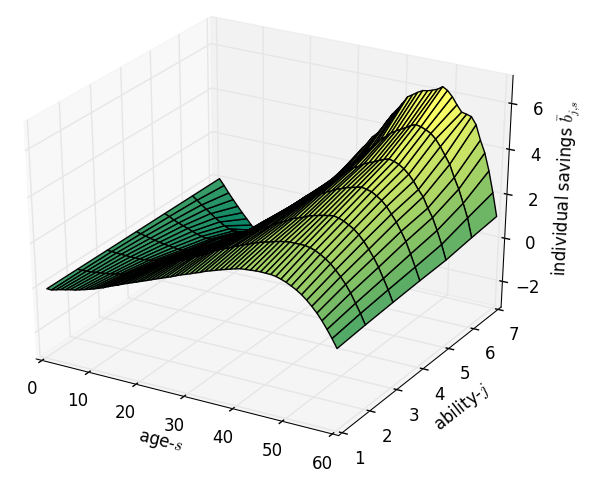
\includegraphics{images/SavSS.png}}}
    \end{figure}

    \begin{figure}[htb]\centering \captionsetup{width=4.0in}
      \caption{\label{FigLabSS}\textbf{Stationary steady-state distribution of individual labor supply $\bar{n}_{j,s}$ for $S=80$ and $J=7$}}
      \fbox{\resizebox{4.0in}{3.0in}{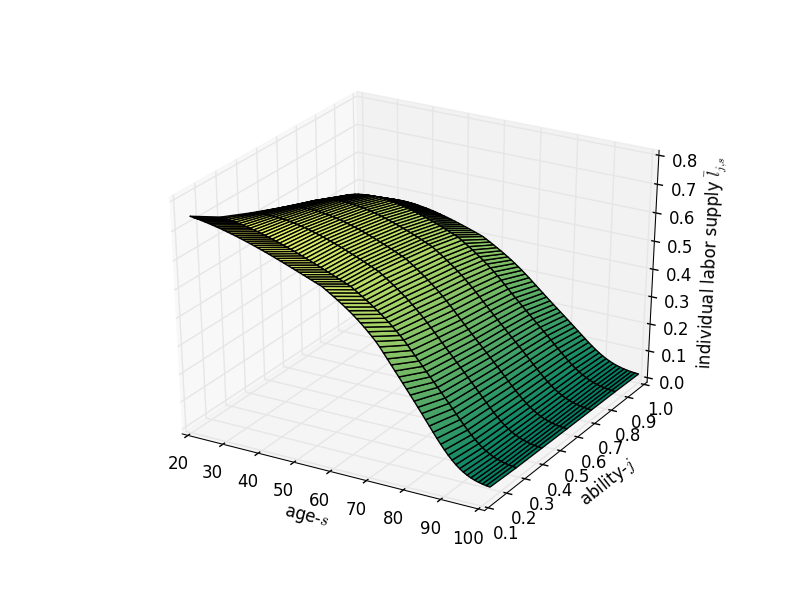
\includegraphics{images/LabSS.png}}}
    \end{figure}

    \begin{figure}[htb]\centering \captionsetup{width=4.0in}
      \caption{\label{FigBeqSS}\textbf{Stationary steady-state distribution of intended bequests $\bar{bq}_{j,E+S+1}$ for $S=80$ and $J=7$}}
      \fbox{\resizebox{4.0in}{3.0in}{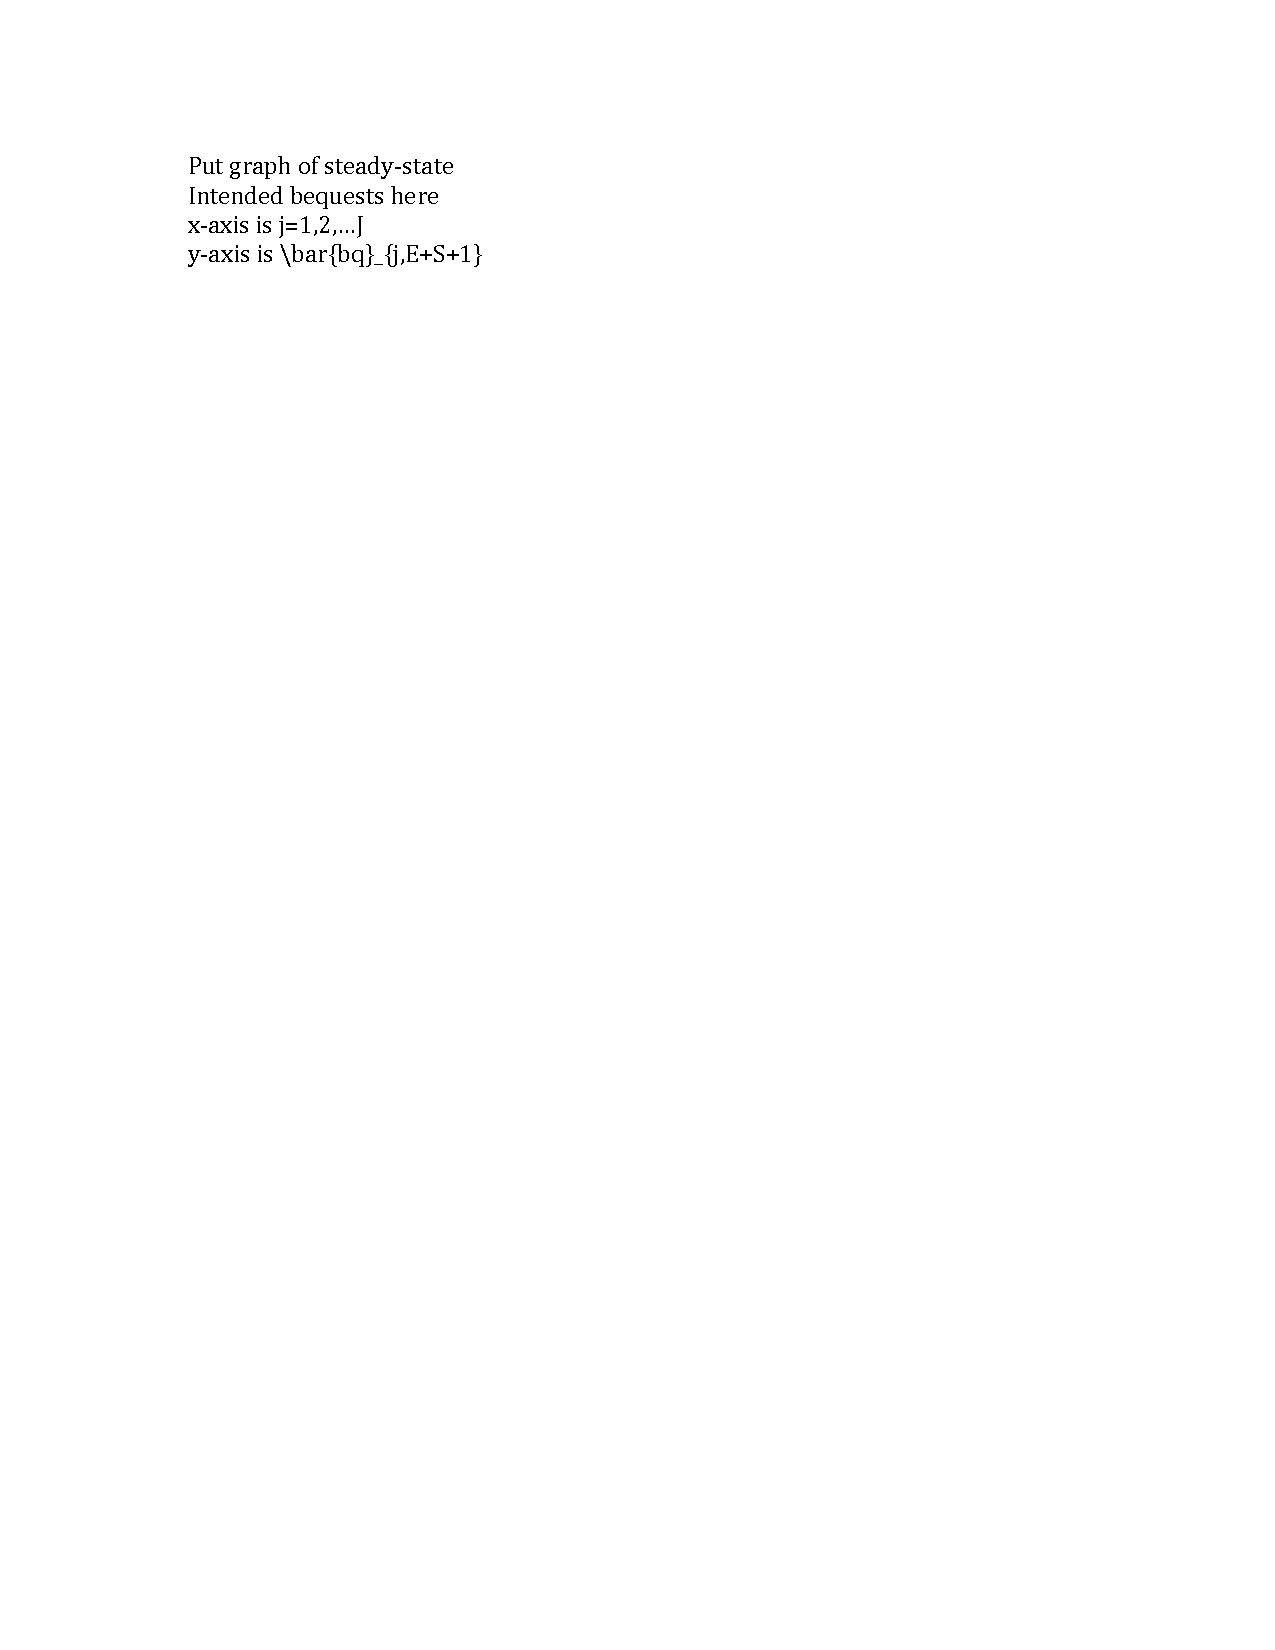
\includegraphics{images/BeqSS.pdf}}}
    \end{figure}

    Figure \ref{FigSavSS} shows the stationary steady-state distribution of individual savings $\bar{b}_{j,s}$, Figure \ref{FigLabSS} shows the stationary steady-state distribution of individual labor supply $\bar{n}_{j,s}$, and Figure \ref{FigBeqSS} shows the steady state distribution of intended bequests $\bar{bq}_{j,E+S+1}$ for a particular calibration of the model described in Table \ref{TabExogVars}. Notice .... %that some intergenerational risk sharing is taking place. Young individuals of high ability, know that they will have high ability and borrow $b_{j,s,t}<0$ in their early years in the steady-state.

    The definition of the stationary non-steady-state equilibrium is similar to Definition \ref{DefEquilSS}, with the stationary steady-state equilibrium definition being a special case of the stationary non-steady-state equilibrium.

    \vspace{7mm}
    \end{spacing}
    \hrule
    \begin{definition}[\textbf{Stationary non-steady-state equilibrium}]\label{DefEquilNonSS}
      A non-autarkic stationary non-steady-state equilibrium in the overlapping generations model with $S$-period lived agents and heterogeneous ability $e_{j,s}$ is defined as allocations $n_{j,s,t}$, $\hat{b}_{j,s+1,t+1}$, and $\hat{bq}_{j,E+S+1,t+1}$ and prices $\hat{w}_t$ and $r_t$ for all $j$, $s$, and $t$ such that the following conditions hold:
       \begin{enumerate}
          \item households have symmetric beliefs $\Omega(\cdot)$ about the evolution of the distribution of savings, and those beliefs about the future distribution of savings equal the realized outcome (rational expectations),
            \begin{equation*}
              \bm{\hat{\Gamma}}_{t+u} = \bm{\hat{\Gamma}}^e_{t+u} = \Omega^u\left( \bm{\hat{\Gamma}}_t\right) \quad\forall t, \quad u\geq 1
            \end{equation*}
          \item households optimize according to \eqref{EqEulerLabStat}, \eqref{EqEulerSavStat}, and \eqref{EqEulerBeqStat}
          \item firms optimize according to \eqref{EqFOCwageStat} and \eqref{EqFOCrate}, and
          \item markets clear according to \eqref{EqMktClrLabStat} and \eqref{EqMktClrCapStat}.
       \end{enumerate}
    \end{definition}
    \hrule
    \begin{spacing}{1.5}
    \vspace{10mm}

    \noindent Taken together, the household labor-leisure and intended bequest decisions in the last period of life show that the optimal labor supply and optimal intended bequests for age $s=E+S$ are each functions of individual holdings of savings, total bequests received, and the prices in that period $n_{j,E+S,t}=\phi\bigl(\hat{b}_{j,E+S,t},\hat{BQ}_{j,t},\hat{w}_t,r_t\bigr)$ and $\hat{bq}_{j,E+S+1,t+1}=\varphi\bigl(\hat{b}_{j,E+S,t},\hat{BQ}_{j,t},\hat{w}_t,r_t\bigr)$. These two decisions are characterized by final-age version of the static labor supply Euler equation \eqref{EqEulerLabStat} and the static intended bequests Euler equation \eqref{EqEulerBeqStat}. Households in their second-to-last period of life in period $t$ have four decisions to make. They must choose how much to work this period $n_{j,E+S-1,t}$ and next period $n_{j,E+S,t+1}$, how much to save this period for next period $\hat{b}_{j,E+S,t+1}$, and how much to bequeath next period $\hat{bq}_{j,E+S+1,t+2}$. The optimal responses for this individual are characterized by the $s=E+S-1$ and $s=E+S$ versions of the static Euler equations \eqref{EqEulerLabStat}, the $s=E+S-1$ version of the intertemporal Euler equation \eqref{EqEulerSavStat}, and the $s=E+S$ static bequest Euler equation \eqref{EqEulerBeqStat}, respectively.

    Optimal savings in the second-to-last period of life $s=E+S-1$ is a function of the current savings as well as the total bequests received and prices in the current period and in the next period $\hat{b}_{j,E+S,t+1} = \psi\bigl(\hat{b}_{j,E+S-1,t},\hat{BQ}_{j,t},\hat{w}_t,r_t,\hat{BQ}_{j,t+1},\hat{w}_{t+1},r_{t+1}|\Omega\bigr)$ given beliefs $\Omega$. As before, the optimal labor supply at age $s=E+S$ is a function of the next period's savings, bequests received, and prices $n_{j,E+S,t+1}=\phi\bigl(\hat{b}_{j,E+S,t+1},\hat{BQ}_{j,t+1},\hat{w}_{t+1},r_{t+1}\bigr)$. But the optimal labor supply at age $s=E+S-1$ is a function of the current savings, current bequests received, and the current prices as well as the future bequests received and future prices because of the dependence on the savings decision in that same period $n_{j,E+S-1,t}=\phi\bigl(\hat{b}_{j,E+S-1,t},\hat{BQ}_{j,t},\hat{w}_t,r_t,\hat{BQ}_{j,t+1},\hat{w}_{t+1},r_{t+1}|\Omega\bigr)$ given beliefs $\Omega$. By induction, we can show that the optimal labor supply, savings, and intended bequests functions for any individual with ability $j$, age $s$, and in period $t$ is a function of current holdings of savings and the lifetime path of total bequests received and prices given beliefs $\Omega$.
    \begin{align}
      n_{j,s,t} &= \phi\Bigl(\hat{b}_{j,s,t},\bigl(\hat{BQ}_{j,v},\hat{w}_v,r_v\bigr)_{v=t}^{t+S-s}|\Omega\Bigr) \quad\forall j,s,t \label{EqLabPolFuncGen} \\
      \hat{b}_{j,s+1,t+1} &= \psi\Bigl(\hat{b}_{j,s,t},\bigl(\hat{BQ}_{j,v},\hat{w}_v,r_v\bigr)_{v=t}^{t+S-s}|\Omega\Bigr) \quad\forall j,t \quad\text{and}\quad 1\leq s\leq S-1 \label{EqSavPolFuncGen} \\
      \hat{bq}_{j,E+S+1,t+1} &= \varphi\Bigl(\hat{b}_{j,s,t},\hat{BQ}_{j,t},\hat{w}_t,r_t\Bigr) \quad\quad\quad\quad\quad\:\:\:\forall j,t \label{EqBeqPolFuncGen}
    \end{align}

    If one knows the current distribution of households savings and intended bequests $\bm{\hat{\Gamma}}_t$ and has a beliefs function that predicts the law of motion over time for $\bm{\hat{\Gamma}}_t$, then one can predict time series for total bequests received $\hat{BQ}_{j,t}$, real wages $\hat{w}_t$ and real interest rates $r_t$ necessary for solving each household's optimal decisions. Characteristic (i) in equilibrium definition \ref{DefEquilNonSS} that individuals be able to forecast prices with perfect foresight over their lifetimes implies that each individual has correct information and beliefs about all the other individuals optimization problems and information. It also implies that the equilibrium allocations and prices are really just functions of the entire distribution of savings at a particular period, as well as a law of motion for that distribution of savings.

    In equilibrium, the steady-state household labor supplies $\bar{n}_{j,s}$ for all $j$ and $s$, the steady-state intended bequests $\bar{bq}_{j,E+S+1}$, the steady-state real wage $\bar{w}$, and the steady-state real rental rate $\bar{r}$ are simply functions of the steady-state distribution of savings $\bar{\Gamma}$. This is clear from the steady-state version of the capital market clearing condition \eqref{EqMktClrCapStat} and the fact that aggregate labor supply is a function of the sum of exogenous efficiency units of labor in the labor market clearing condition \eqref{EqMktClrLabStat}. And the two firm first order conditions for the real wage $\hat{w}_t$ \eqref{EqFOCwageStat} and real rental rate $r_t$ \eqref{EqFOCrate} are only functions of the aggregate capital stock $\hat{K}_t$ and aggregate labor $\hat{L}_t$.

    \begin{figure}[htb]\centering \captionsetup{width=4.0in}
      \caption{\label{FigKpathTPI}\textbf{Equilibrium time path of $K_t$ for $S=60$ and $J=7$}}
      \fbox{\resizebox{4.0in}{3.0in}{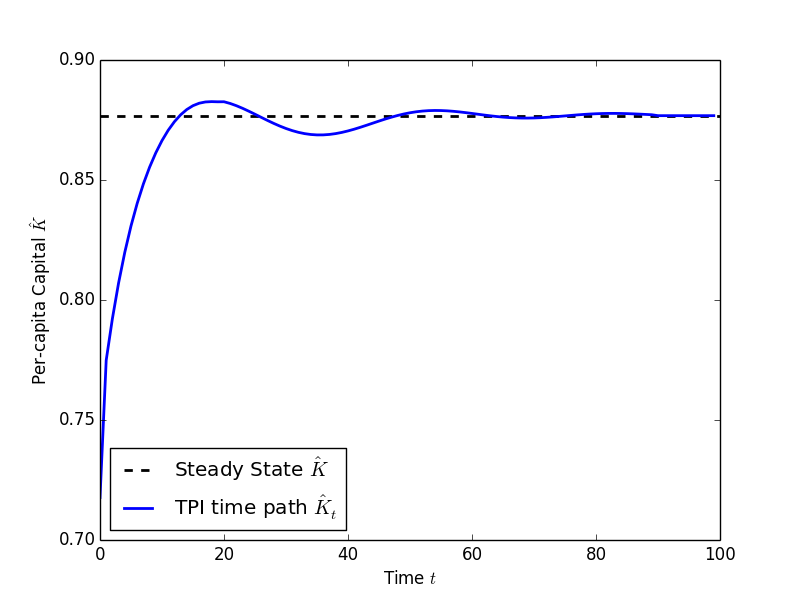
\includegraphics{images/KpathTPI.png}}}
    \end{figure}

    \begin{figure}[htb]\centering \captionsetup{width=4.0in}
      \caption{\label{FigLpathTPI}\textbf{Equilibrium time path of $L_t$ for $S=60$ and $J=7$}}
      \fbox{\resizebox{4.0in}{3.0in}{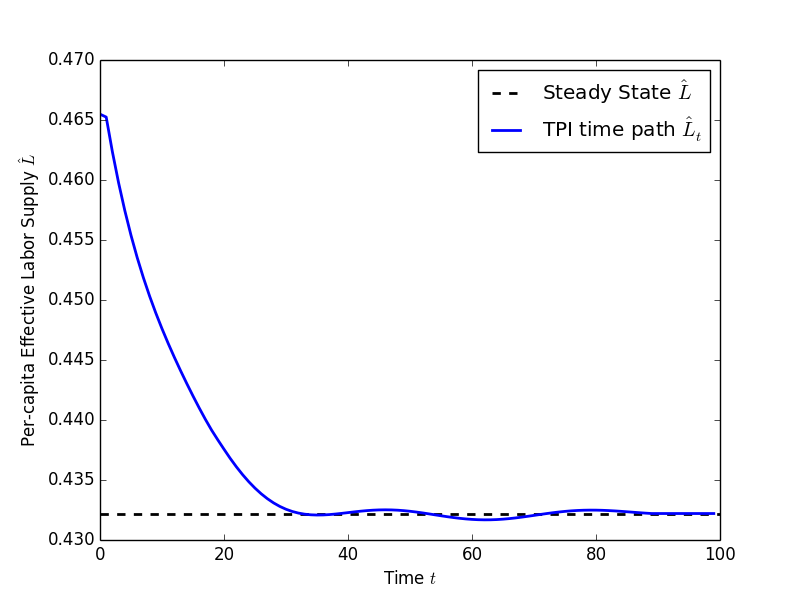
\includegraphics{images/LpathTPI.png}}}
    \end{figure}

    To solve for any stationary non-steady-state equilibrium time path of the economy from an arbitrary current state to the steady state, we follow the time path iteration (TPI) method of \citet{AuerbachKotlikoff:1987}. Appendix \ref{AppNonSSsolve} details how to solve for the non-steady-state equilibrium time path using the TPI method. The approach is to choose an arbitrary time path for the stationary aggregate capital stock $\hat{K}_t$, stationary aggregate labor $\hat{L}_t$, and total bequests received $\hat{BQ}_{j,t}$ for each type $j$. This initial guess of a path implies arbitrary beliefs that violate the rational expectations requirement. We then solve for households' optimal decisions given the time paths of those variables, which decisions imply new time paths of those variables. We then update the time path as a convex combination of the initial guess and the new implied path. Figure \ref{FigKpathTPI} shows the equilibrium time path of the aggregate capital stock for the calibration used in Figure \ref{FigKpathTPI} for $T=80$ periods starting from an initial distribution of savings in which $b_{j,s,1}=(0.9\bar{K})/[(S-1)J]$ for all $j$ and $s$. We used $\nu=0.2$ as our time-path updating dampening parameter (see Equation \eqref{EqTPInewpath} in Appendix \ref{AppNonSSsolve}.)


\clearpage

\end{spacing}

\newpage
\renewcommand{\theequation}{A.\arabic{section}.\arabic{equation}}
                                                 % redefine the command that creates the section number
\renewcommand{\thesection}{A-\arabic{section}}   % redefine the command that creates the equation number
\setcounter{equation}{0}                         % reset counter
\setcounter{section}{0}                          % reset section number
\section*{APPENDIX}                              % use *-form to suppress numbering


\section{Characteristics of exogenous population growth assumptions}\label{AppPopGrowth}

  In this appendix, we describe in detail the exogenous population growth assumptions in the model and their implications. In Section \ref{SecIndProb}, we define the laws of motion for the population of each cohort $\omega_{s,t}$ to be the following.
  \begin{equation}\tag{\ref{EqPopLawofmotion}}
    \begin{split}
      \omega_{1,t+1} &= \sum_{s=1}^{E+S} f_s\omega_{s,t}\quad\forall t \\
        \omega_{s+1,t+1} &= (1 + i_s - \rho_s)\omega_{s,t}\quad\forall t\quad\text{and}\quad 1\leq s \leq E+S-1
    \end{split}
  \end{equation}
  We can transform the nonstationary equations in \eqref{EqPopLawofmotion} into stationary laws of motion by dividing both sides by the total populations $N_t$ and $N_{t+1}$ in both periods,
  \begin{equation}\label{EqPopLawofmotionStat}
    \begin{split}
      \hat{\omega}_{1,t+1} &= \frac{\sum_{s=1}^{E+S} f_s\hat{\omega}_{s,t}}{1+g_{n,t+1}}\quad\forall t \\
      \hat{\omega}_{s+1,t+1} &= \frac{(1 + \phi_s - \rho_s)\hat{\omega}_{s,t}}{1+g_{n,t+1}}\quad\forall t\quad\text{and}\quad 1\leq s \leq E+S-1
    \end{split}
  \end{equation}
  where $\hat{\omega}_{s,t}$ is the percent of the total population in age cohort $s$ and the population growth rate $g_{n,t+1}$ between periods $t$ and $t+1$ is defined in \eqref{EqPopGrowth},
  \begin{equation}\label{EqPopLOMbig}
    \scriptsize{\begin{bmatrix}
      \hat{\omega}_{1,t+1} \\ \hat{\omega}_{2,t+1} \\ \hat{\omega}_{2,t+1} \\ \vdots \\ \hat{\omega}_{E+S-1,t+1} \\ \hat{\omega}_{E+S,t+1}
    \end{bmatrix} = \frac{1}{1 + g_{n,t+1}}
    \begin{bmatrix}
      f_1 & f_2 & f_3 & \hdots & f_{E+S-1} & f_{E+S} \\
      1+i_1-\rho_1 & 0 & 0 & \hdots & 0 & 0 \\
      0 & 1+i_2-\rho_2 & 0 & \hdots & 0 & 0 \\
      0 & 0 & 1+i_3-\rho_3 & \hdots & 0 & 0 \\
      \vdots & \vdots & \vdots & \ddots & \vdots & \vdots \\
      0 & 0 & 0 & \hdots & 0 & 0 \\
      0 & 0 & 0 & \hdots & 1+i_{E+S-1}-\rho_{E+S-1} & 0
    \end{bmatrix}
    \begin{bmatrix}
      \hat{\omega}_{1,t} \\ \hat{\omega}_{2,t} \\ \hat{\omega}_{2,t} \\ \vdots \\ \hat{\omega}_{E+S-1,t} \\ \hat{\omega}_{E+S,t}
    \end{bmatrix}}
  \end{equation}
  where we restrict $1+i_s-\rho_s\geq 0$ for all $s$.

  We write \eqref{EqPopLOMbig} in matrix notation as the following.
  \begin{equation}\label{EqPopLOMmat}
    \bm{\hat{\omega}}_{t+1} = \frac{1}{1+g_{n,t+1}}\bm{\Omega}\bm{\hat{\omega}}_t \quad\forall t
  \end{equation}
  The stationary steady state population distribution $\bm{\bar{\omega}}$ is the eigenvector $\bm{\omega}$ with eigenvalue $(1+\bar{g}_n)$ of the matrix $\bm{\Omega}$ that satisfies the following version of \eqref{EqPopLOMmat}.
  \begin{equation}\label{EqPopLOMss}
    (1+\bar{g}_n)\bm{\bar{\omega}} = \bm{\Omega}\bm{\bar{\omega}}
  \end{equation}

  \noindent TODO:
  \begin{itemize}
    \item We need to show the conditions under which the matrix $\bm{\Omega}$ has only one eigenvector associated with one positive eigen value with no complex part.
    \item Another approach is to simply simulate the problem from the initial population distribution $\bm{\omega}_0$ and what the steady state $\bm{\bar{\omega}}$ is and how many periods it takes to get there.
      \begin{itemize}
        \item We can use the number of periods to arrive at the steady state as a lower bound for $T$ in the time path iteration algorithm.
      \end{itemize}
  \end{itemize}

  Because the population growth process is exogenous to the model, we calibrate it to annual age data for age years $s=1$ to $s=100$. As is shown in Figure \ref{FigPerTime}, period $s=1$ corresponds to the first year of life between birth and when an individual turns one year old.

  \begin{figure}[htbp]\centering \captionsetup{width=4.0in}
    \caption{\label{FigPerTime}\textbf{Correspondence of model timing to data timing for model periods of one year}}
    \fbox{\resizebox{4.0in}{2.3in}{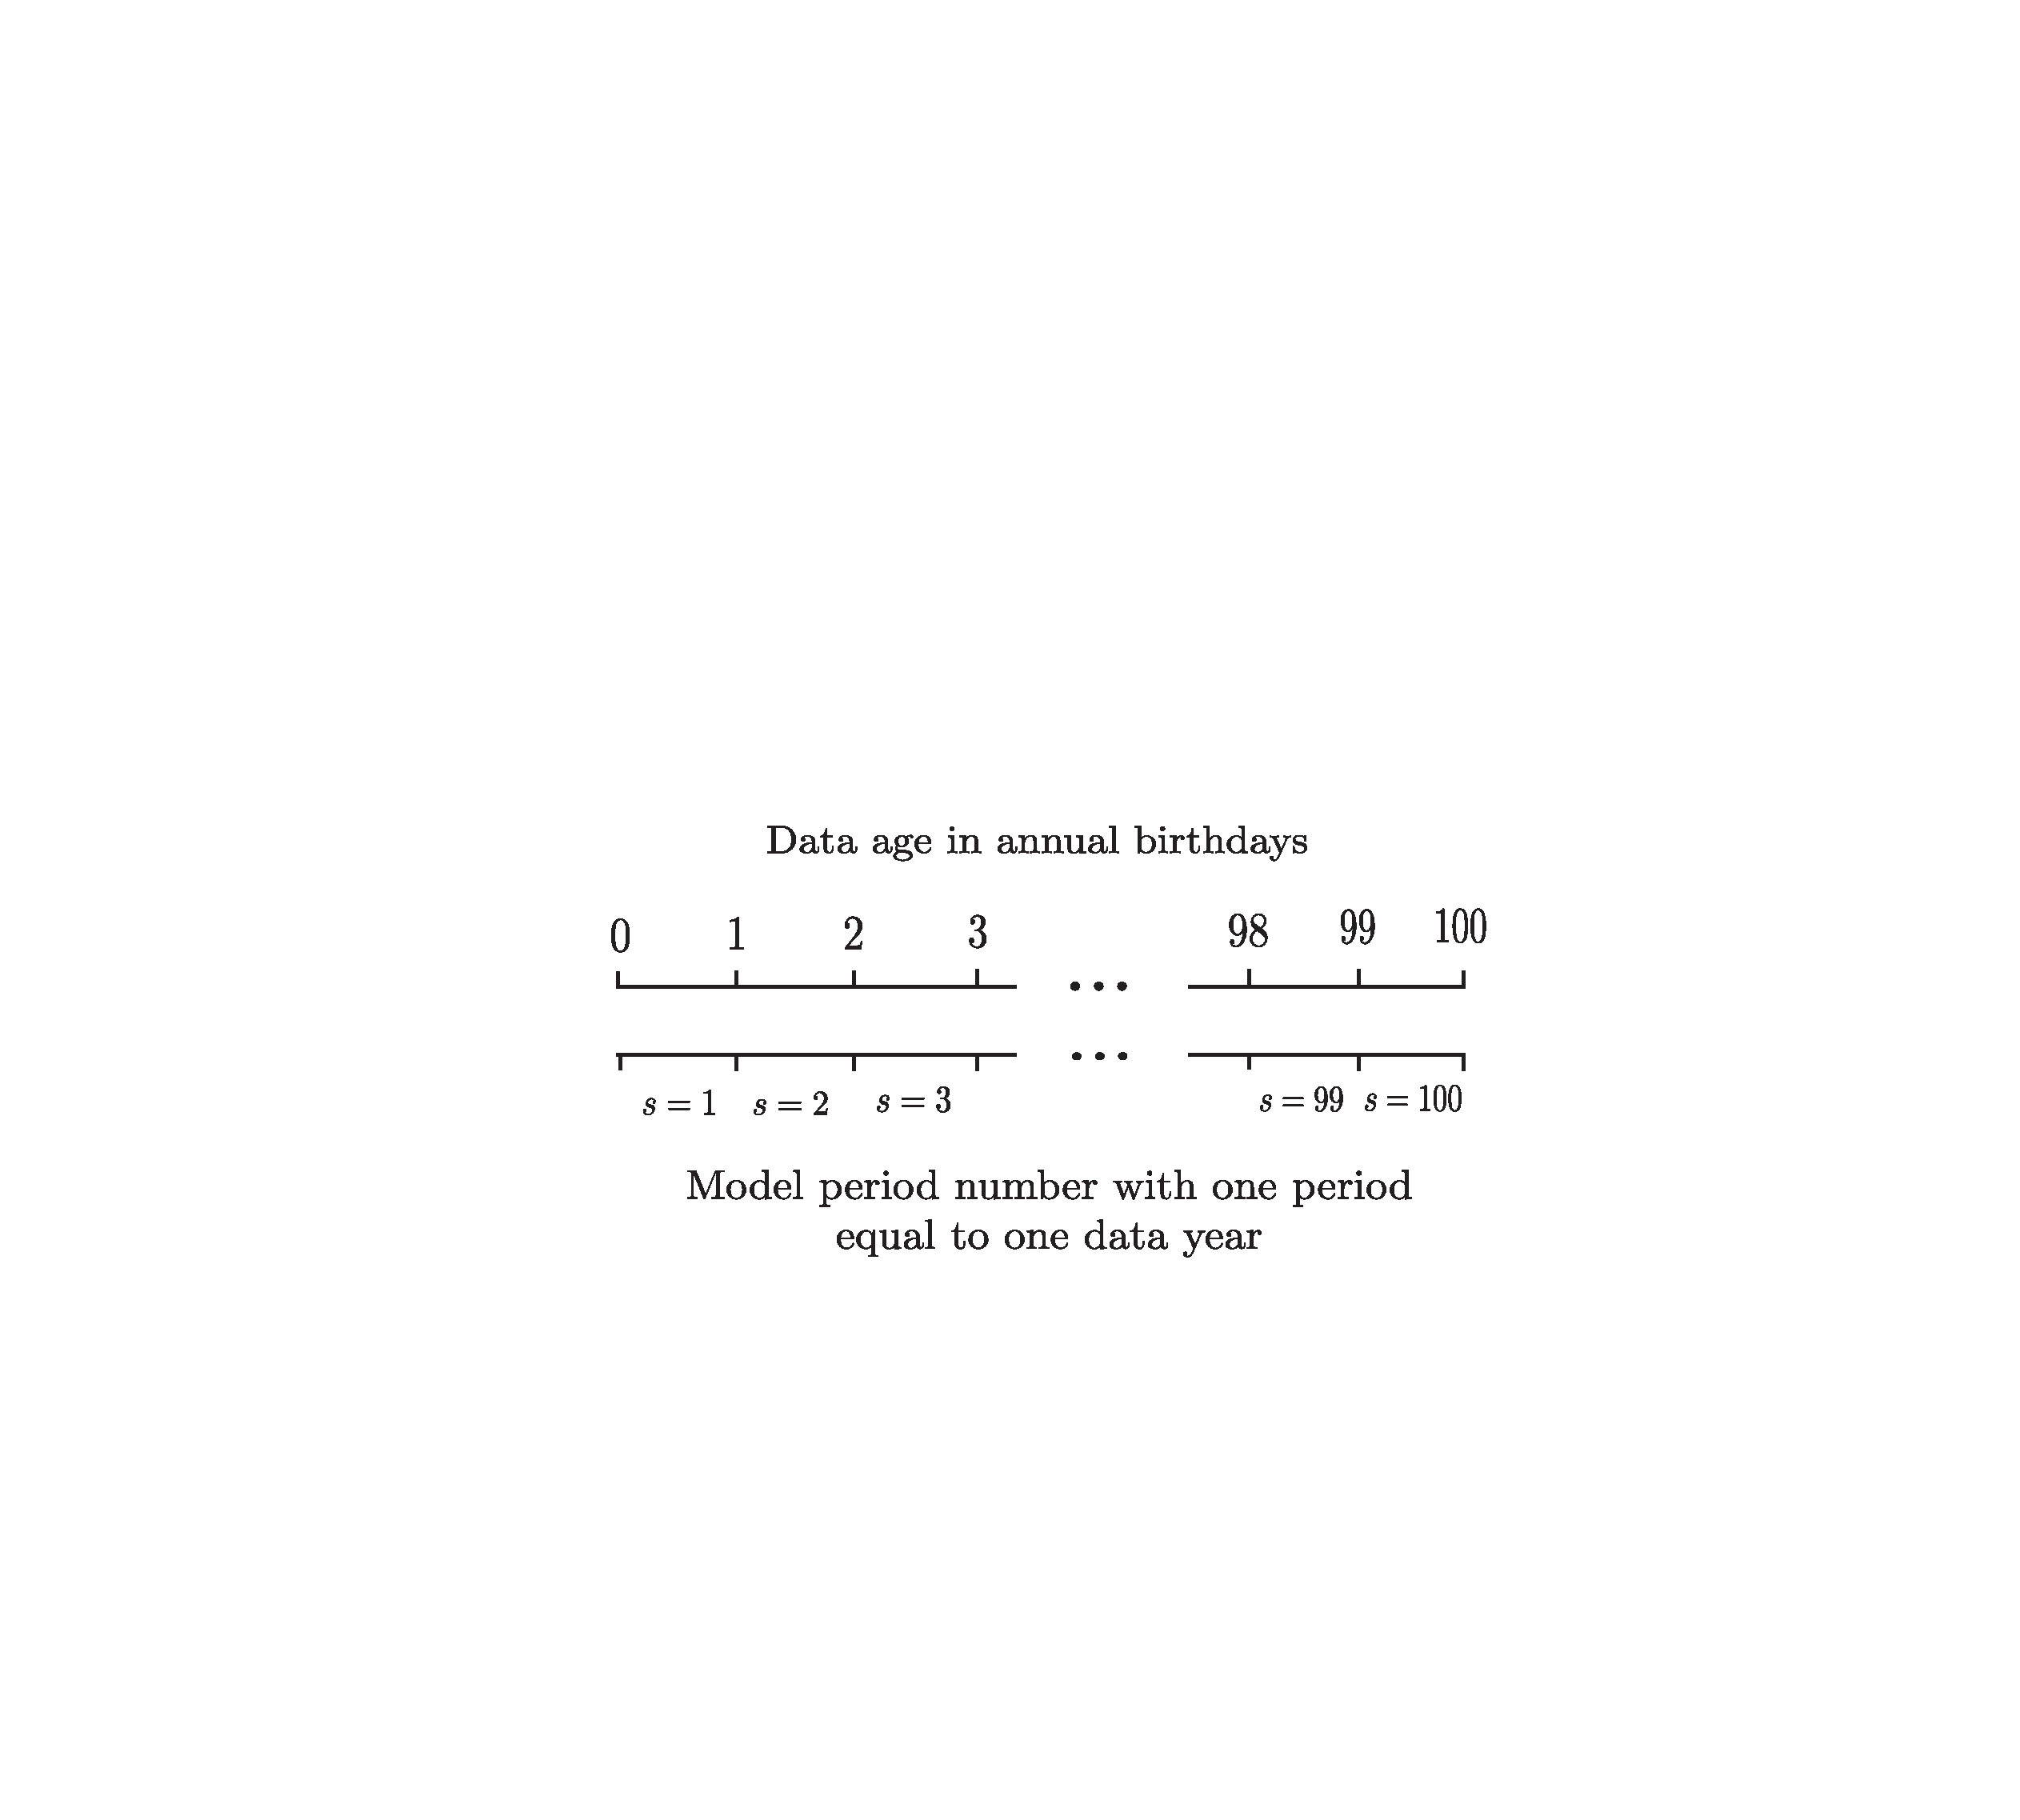
\includegraphics{images/FigPerTime.pdf}}}
  \end{figure}

  Our initial population distribution $\{\omega_{s,1}\}_{s=1}^{100}$ in Figure \ref{FigInitPopDist} comes from \citet{Census:2014} population estimates for both sexes for 2013. The fertility rates $\{f_s\}_{s=1}^{100}$ in Figure \ref{FigFertRates} come from \citet[Table 1]{NVSR:2010}. The mortality rates $\{\rho_s\}_{s=1}^{99}$ in Figure \ref{FigMortRates} come from the 2010 death probabilities in \citet{SocSec:2010}. We enforce a strict mortality rate of $\rho_{100}=1$ in our model.

  \begin{figure}[htbp]\centering \captionsetup{width=4.0in}
    \caption{\label{FigInitPopDist}\textbf{Initial population distribution $\omega_{s,1}$ by year, $1\leq s\leq 100$}}
    \fbox{\resizebox{4.0in}{2.8in}{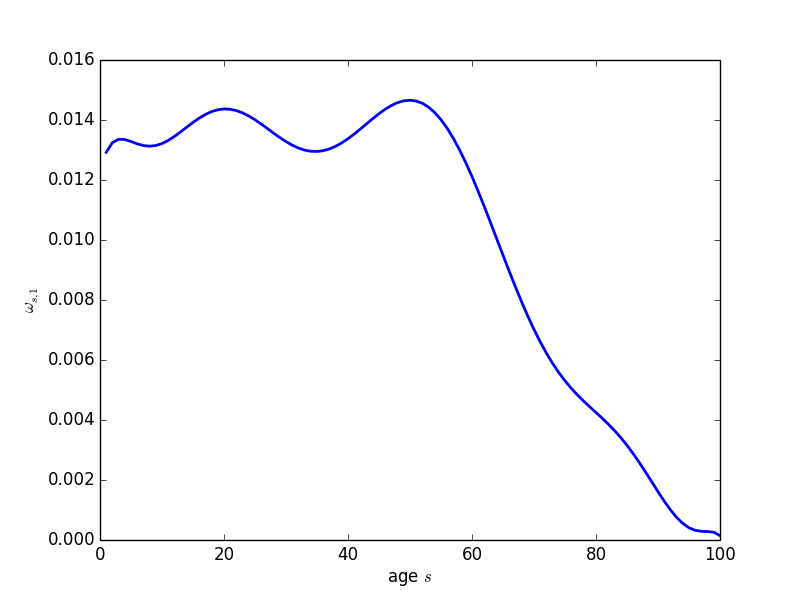
\includegraphics{images/omega_init.png}}}
  \end{figure}

  \begin{figure}[htbp]\centering \captionsetup{width=4.0in}
    \caption{\label{FigFertRates}\textbf{Fertility rates $f_s$ by year, $1\leq s\leq 100$}}
    \fbox{\resizebox{4.0in}{2.8in}{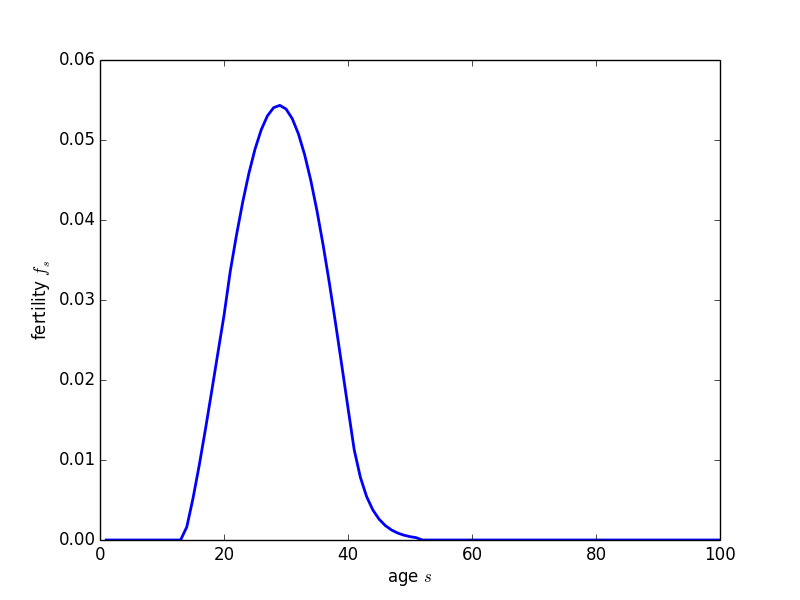
\includegraphics{images/fert_rates.png}}}
  \end{figure}

  \begin{figure}[htbp]\centering \captionsetup{width=4.0in}
    \caption{\label{FigMortRates}\textbf{Mortality rates $\rho_s$ by year, $1\leq s\leq 100$}}
    \fbox{\resizebox{4.0in}{2.8in}{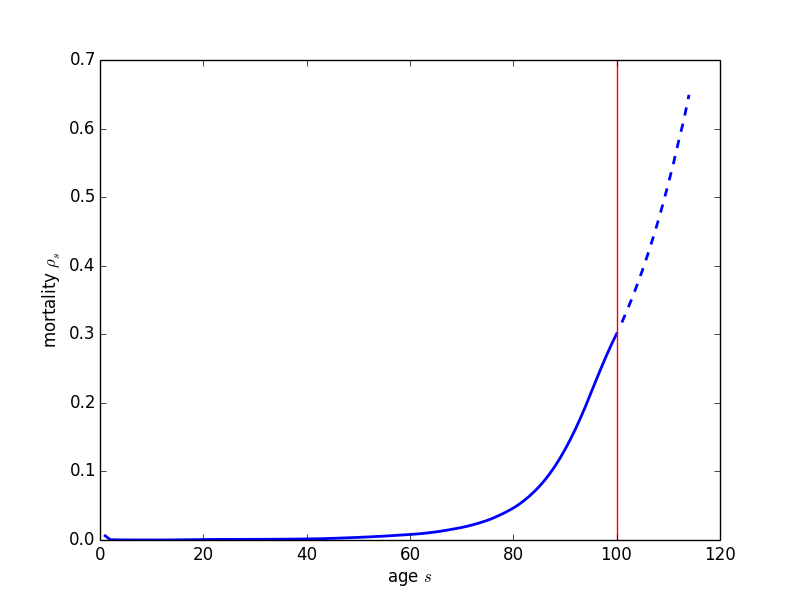
\includegraphics{images/mort_rates.png}}}
  \end{figure}

  The immigration rates $\{i_s\}_{s=1}^{99}$ in Figure \ref{FigImmigRates} are essentially residuals. We take total population for two consecutive years $N_t$ and $N_{t+1}$ and the population distribution by age in both of those years $\bm{\omega}_{t}$ and $\bm{\omega}_{t+1}$from the \citet{Census:2014} data. We then deduce the immigration rates $\{i_s\}_{s=1}^{99}$ using equation \eqref{EqPopLawofmotionStat}. We do this for three consecutive sets of years, so that our calibrated immigration rates by age are the average of our three years of deduced rates from the data for each age.

  \begin{figure}[htbp]\centering \captionsetup{width=4.0in}
    \caption{\label{FigImmigRates}\textbf{Immigration rates $i_s$ by year, $1\leq s\leq 100$}}
    \fbox{\resizebox{4.0in}{2.8in}{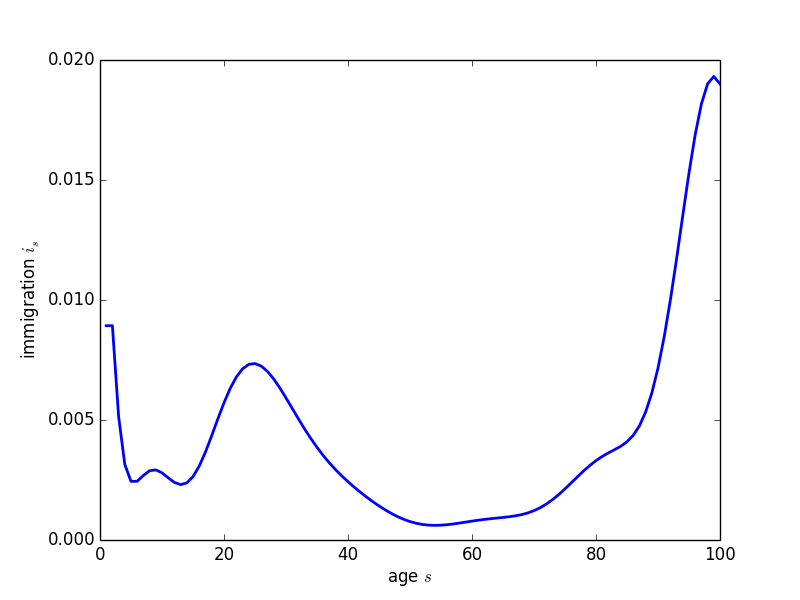
\includegraphics{images/imm_rates.png}}}
  \end{figure}

  Figure \ref{FigPopPath} shows the predicted time path of the total population $N_t$ given $\omega_{s,1}$ $f_s$, $i_s$, and $\rho_s$. Notice that the population approaches a constant growth rate. This is a result of the stationary population percent distribution $\bm{\bar{\omega}}$ eventually being reached. Figure \ref{FigSSpopdist} shows the steady-state population percent distribution by age $\bm{\bar{\omega}}$.

  \begin{figure}[htbp]\centering \captionsetup{width=4.0in}
    \caption{\label{FigPopPath}\textbf{Forecast time path of population growth rate $g_{n,t}$}}
    \fbox{\resizebox{4.0in}{2.8in}{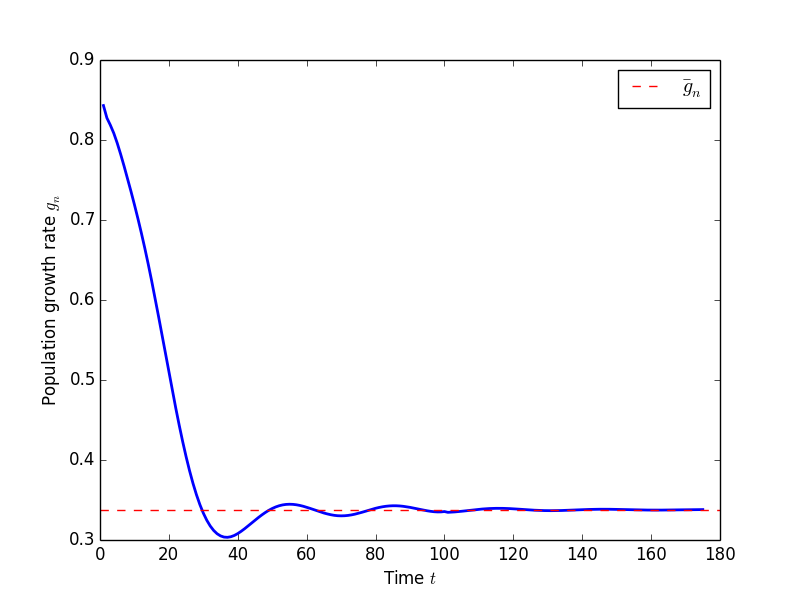
\includegraphics{images/Population_growthrate.png}}}
  \end{figure}

  \begin{figure}[htbp]\centering \captionsetup{width=4.0in}
    \caption{\label{FigSSpopdist}\textbf{Steady-state population percent distribution by age $\bm{\bar{\omega}}$}}
    \fbox{\resizebox{4.0in}{2.8in}{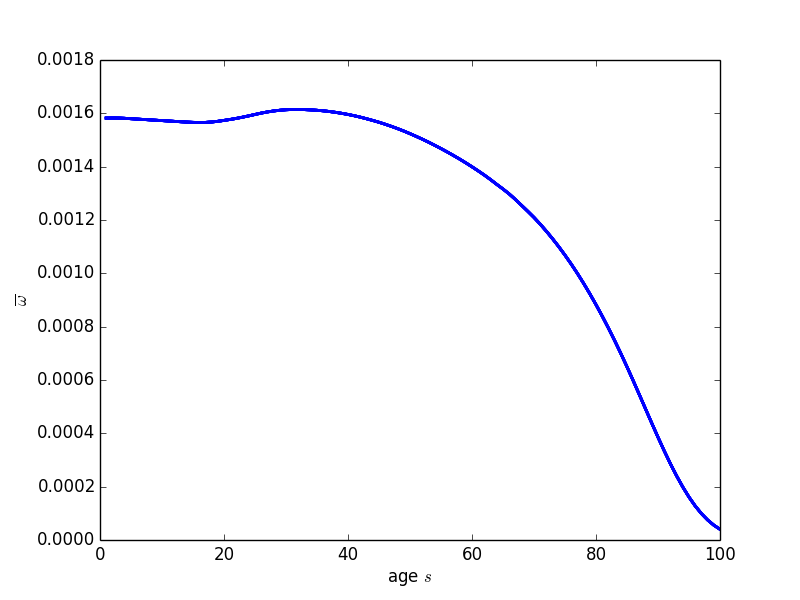
\includegraphics{images/omega_ss.png}}}
  \end{figure}
  \clearpage


\newpage
\section{Calibration of ability process}\label{AppAbilCalib}

  \setcounter{equation}{0}

  There are two pieces to the calibration of the deterministic ability process $e_{j,s}$. The population percentage in each of the $j$ ability types is $\lambda_j>0$ such that $\sum_{j=1}^J \lambda_j = 1$. In this paper, we assume that all the ability types have equal measure $\lambda_j= 1/J$ for all $j$. However, we could easily change the percentile size if we were interested in particular quantiles of the ability distribution or income distribution.

  The calibration of the ability process $e_{j,s}$ is as follows.  First, the ability types themselves must be calibrated. For each age group $s \in S$, the hourly wage rates are sorted into $J$ percentile groups.  The ability type for each percentile group is the mean wage for the percentile group, normalized by the average wage of all individuals in the data set.

  The data used to calibrate the ability types were obtained from the Current Population Survey.\footnote{U.S. Census Bureau, Dataferret, Current Population Survey, 2014. The variables $PRTAGE$, $PTERNHLY$, and $PWCMPWGT$ were used for the age, hourly wage rate, and population weight of individuals, respectively. \\ [-2pt]} A polynomial is fit to the wage data for individuals age 20 to 70.  For lack of hourly wage data from the elderly, wages for individuals age 71 to 100 are extrapolated using a simple exponential function. This was done for each percentile group.  Due to a limited number of observations in the survey who included their hourly wage, data was taken from the months of January, February, March, April, and May 2014.  Population weights were also used to obtain the correct percentile groups of individuals.  The income levels for the $J$ ability types were then calculated for each month, and then an average was taken of the five calibrations of the ability types in order to produce a final calibration to be used in the model. Figure \ref{FigAbility} shows this income distribution across age and ability type.

    \begin{figure}[htb]\centering \captionsetup{width=4.0in}
      \caption{\label{FigAbility}\textbf{Distribution of Income where $S=80$ and $J=7$}}
      \fbox{\resizebox{4.0in}{2.8in}{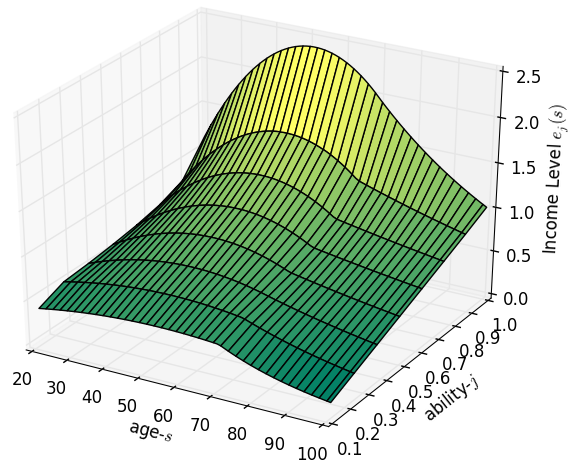
\includegraphics{images/ability.png}}}
    \end{figure}

  In this paper, individuals are assigned ability types at the beginning of their life, and cannot change types later on.
  \clearpage


\newpage
\section{Calibration of disutility of labor parameter to match labor supply}\label{AppDisutilLab}

  \setcounter{equation}{0}

  The household period utility function in \eqref{EqUtilMax} has a linearly separable term for the utility of labor. Conversely, it represents the disutility of labor.
  \begin{equation}\label{EqPerUtil}
    u\left(c_{j,s,t},n_{j,s,t}\right) =
      \begin{cases}
        \frac{\left(c_{j,s,t}\right)^{1-\sigma} - 1}{1-\sigma} + \chi_{n,s} e^{g_y t(1-\sigma)}\frac{(\tilde{l}-n_{j,s,t})^{1-\eta}}{1-\eta} \quad\text{if}\quad E+1\leq s \leq E+S-1 \\
        \frac{\left(c_{j,s,t}\right)^{1-\sigma} - 1}{1-\sigma} + \chi_{n,s} e^{g_y t(1-\sigma)}\frac{(\tilde{l}-n_{j,s,t})^{1-\eta}}{1-\eta} + \chi_b\frac{\left(bq_{j,s+1,t+1}\right)^{1-\sigma} - 1}{1-\sigma} \\
        \quad\quad\quad\quad\quad\quad\quad\quad\quad\quad\quad\quad\quad\quad\quad\:\:\:\text{if}\quad s=E+S
      \end{cases}
  \end{equation}
  The disutility of labor term in the period utility function is primarily characterized by two parameters. The parameter $\eta>1$ is proportional to the Frisch elasticity of labor supply, and $\chi_{n,s}>0$ sets the level of the disutility of labor (utility of leisure).

  In calibrating the model, we get a strange steady-state equilibrium distribution of labor supply by age if we make $\chi_{n,s}$ constant for all ages. As can be seen in Figure \ref{FigMortRates} in Appendix \ref{AppPopGrowth}, mortality hazard rates really start to rise at age 65. If we make the disutility of labor constant across the life cycle, we see too much labor supply in old age among households between ages 70 and 100.

  The intuition is simple. If the disutility of labor is constant across the life cycle, agents who live beyond age 80 are surprised to some degree, and their ability is decreasing as can be seen in Figure \ref{FigAbility}. These forces together mean that the surviving household needs to smooth consumption more and does not have enough savings to do so. For this reason, they work more to keep their consumption at a steady level.

  This result is counterfactual. Further, it is likely that the disutility of labor is not constant across the lifecycle. Market work becomes more onerous as households age. For this reason, we implement a calibration of $\chi_{n,s}$ in which it is constant $\chi_n>0$ for model ages corresponding to ages 21 through 65 and increases exponentially thereafter.
  \begin{equation}\label{EqChi_ns}
    \chi_{n,s} =
      \begin{cases}
        \chi_n \quad\quad\quad\quad\quad\quad\quad\quad\quad\quad\quad\quad\:\:\:\text{if}\quad E+1\leq s\leq E+\text{round}\left(\frac{9}{16}S\right) \\
        \chi_n + \left[s-E-\text{round}\left(\frac{9}{16}S\right)\right]^2 \quad\text{if}\quad E+\text{round}\left(\frac{9}{16}S\right) + 1 \leq s \leq E+S
      \end{cases}
  \end{equation}
  This exogenously exponentially increasing disutility of labor after age 65 induces a smooth degree of retirement that is more consistent with the empirical labor supply at those ages.


\newpage
\section{Stationary constraints on individual borrowing}\label{AppBorConstr}

  \setcounter{equation}{0}

  As described in Section \ref{SecIndProb}, individuals are allowed to borrow $b_{j,s,t}<0$ for some $j$ and $s$ in period $t$. However, two constraints must hold. First, the individual must be able to pay back the balance with interest $r_{t+1}$ in the next period without driving consumption in the next period $c_{j,s+1,t+1}$ to be nonpositive. Let $\tilde{b}_{j,s,t}$ be the minimum stationary value of savings in a period.
  \begin{equation}\label{EqSavMin}
    \hat{b}_{j,s,t}\geq\tilde{b}_{j,s,t} \quad\forall j,s,t
  \end{equation}
  Rearranging the stationary versions of the bugdet constraints in \eqref{EqBC1}, \eqref{EqBC2}, and \eqref{EqBC3} and using backward induction gives the following expressions for $\tilde{b}_{j,s,t}$,
  \begin{equation}\label{EqBorConsts}
    \begin{split}
      \tilde{b}_{j,E+S,t} &= \frac{\tilde{c} + \tilde{bq} - \hat{w}_t e_{j,E+S}\tilde{l} - \frac{\hat{BQ}_{j,t}}{\lambda_j}}{1+r_t}  \\
      \tilde{b}_{j,E+S-1,t-1} &= \frac{\tilde{c} + e^{g_y}\tilde{b}_{j,E+S,t} - \hat{w}_{t-1}e_{j,E+S-1}\tilde{l} - \frac{\hat{BQ}_{j,t-1}}{\lambda_j}}{1+r_{t-1}} \\
      &\vdots \\
      \tilde{b}_{j,E+2,t-S+2} &= \frac{\tilde{c} + e^{g_y}\tilde{b}_{j,E+3,t-S+3} - \hat{w}_{t-S+2}e_{j,E+2}\tilde{l} - \frac{\hat{BQ}_{j,t-S+2}}{\lambda_j}}{1+r_{t-S+2}}
    \end{split}
  \end{equation}
  where $\tilde{c}>0$ and $\tilde{bq}>0$ are some minimum amount of stationary consumption and stationary intended bequests, respectively, and $\tilde{l}$ is the maximum amount an individual can work from the time constraint \eqref{EqLabConstr}. With endogenous labor supply $n_{j,s,t}$, it is less likely that the individual borrowing constraints ever bind. This is because the disutility of labor increases exponentially according to $\eta>1$ in the period utility function \eqref{EqUtilMax}.

  In addition to the individual borrowing constraint \eqref{EqSavMin}, a strict aggregate borrowing constraint must be met. That is, the stationary aggregate capital stock must be strictly positive.
  \begin{equation}\label{EqAggrCapConstr}
    \hat{K}_t > 0 \quad\forall t
  \end{equation}

  Lastly, because households can borrow, some individual unintended bequests in a given period can be negative. That is, households can bequeath debt as well as savings. We require that total unintended and intended bequests for all types $j$ in all periods $t$ characterized in \eqref{EqTotBeq} must be nonegative $BQ_{j,t}\geq 0$. However, this constraint will never bind if the aggregate capital constraint $K_t>0$ in \eqref{EqAggrCapConstr} holds.


\newpage
\section{Solving for stationary steady-state equilibrium}\label{AppSSsolve}

  \setcounter{equation}{0}
  \renewcommand\theenumi{\arabic{enumi}}
  \renewcommand\theenumii{\alph{enumii}}
  \renewcommand\theenumiii{\roman{enumiii}}

  This section describes the solution method for the stationary steady-state equilibrium described in Definition \ref{DefEquilSS}.

  \begin{enumerate}
    \item Use the techniques in Appendix \ref{AppPopGrowth} to solve for the steady-state population distribution vector $\bm{\bar{\omega}}$ of the exogenous population process.
    \item Choose an initial guess for the stationary steady-state distribution of capital $\bar{b}_{j,s+1}$ for all $j$ and $s=E+2,E+3,...E+S$, labor supply $\bar{n}_{j,s}$ for all $j$ and $s$, and intended bequests $\bar{bq}_{j,E+S+1}$ for all $j$.
      \begin{itemize}
        \item A good first guess is a large positive number for all the $\bar{n}_{j,s}$ that is slightly less than $\tilde{l}$ and to choose some small positive number for $\bar{b}_{j,s+1}$ and $\bar{bq}_{j,E+S+1}$ that is small enough to be less than the minimum income that an individual might have $\bar{w}e_{j,s}\bar{n}_{j,s}$.
      \end{itemize}
    \item Perform a constrained root finder that chooses $\bar{b}_{j,s+1}$, $\bar{n}_{j,s}$, and $\bar{bq}_{j,E+S+1}$ that solves the $2JS$ stationary steady-state Euler equations \eqref{EqEulerLabSS}, \eqref{EqEulerSavSS}, and \eqref{EqEulerBeqSS}.
    \item Make sure none of the implied steady-state consumptions $\bar{c}_{j,s}$ is less-than-or-equal-to zero.
      \begin{itemize}
        \item If one consumption is less-than-or-equal-to zero $\bar{c}_{j,s}\leq 0$, then try different starting values.
      \end{itemize}
    \item Make sure that none of the Euler errors is too large in absolute value for interior stationary steady-state values. A steady-state Euler error is the following, which is supposed to be close to zero for all $j$ and $s$:
      \begin{equation}\label{EqSSeulerrLab}
        \frac{\chi_{n,s}\left(\tilde{l}-\bar{n}_{j,s}\right)^{-\eta}}{\bar{w}e_{j,s}\left(\bar{c}_{j,s}\right)^{-\sigma}} - 1 \quad\quad\quad\quad\quad\quad\quad\forall j\quad\text{and}\quad E+1\leq s\leq E+S
      \end{equation}
      \begin{equation}\label{EqSSeulerrSav}
        \frac{\beta\left(1-\rho_s\right)\left(1+\bar{r}\right)e^{-\sigma g_y}\left(\bar{c}_{j,s+1}\right)^{-\sigma}}{\left(\bar{c}_{j,s}\right)^{-\sigma}} - 1 \quad\forall j\quad\text{and}\quad E+1\leq s\leq E+S-1
      \end{equation}
      \begin{equation}\label{EqSSeulerrBeq}
        \frac{\chi_b e^{-\sigma g_y}\left(\bar{bq}_{j,E+S+1}\right)^{-\sigma}}{\left(\bar{c}_{j,E+S}\right)^{-\sigma}} - 1 \quad\quad\quad\forall j\quad\quad\quad\quad\quad\quad\quad\quad\quad\quad
      \end{equation}
    \item Make sure that the unconstrained solution satisfies the individual borrowing constraints in \eqref{EqSavMin} and \eqref{EqBorConsts}.
      \begin{itemize}
        \item If any individual's borrowing constraint is not satisfied using the unconstrained root finding operation, rerun the root finding operation in step (3) as a constrained minimization problem with the borrowing constraints imposed on those individuals.
        \item Repeat steps (3) through (6) until all the individual borrowing constraints are met.
      \end{itemize}
    \item Make sure that the solution satisfies the aggregate borrowing constraint \eqref{EqAggrCapConstr}.
      \begin{itemize}
        \item If it does not, use the least distortionary upward adjustment to individual steady-state savings $\bar{b}_{j,s+1}$?
      \end{itemize}
  \end{enumerate}


\newpage
\section{Solving for stationary non-steady-state equilibrium by time path iteration}\label{AppNonSSsolve}

  \setcounter{equation}{0}

  This section outlines the benchmark time path iteration (TPI) method of \citet{AuerbachKotlikoff:1987} for solving the stationary non-steady-state equilibrium transition path of the distribution of savings. TPI finds a fixed point for the transition path of the distribution of capital for a given initial state of the distribution of capital. The idea is that the economy is infinitely lived, even though the agents that make up the economy are not. Rather than recursively solving for equilibrium policy functions by iterating on individual value functions, one must recursively solve for the policy functions by iterating on the entire transition path of the endogenous objects in the economy (see \citet[ch. 17]{StokeyLucas:1989}).

  The key assumption is that the economy will reach the steady-state equilibrium described in Definition \ref{DefEquilSS} in a finite number of periods $T<\infty$ regardless of the initial state. Let $\bm{\hat{\Gamma}}_t$ represent the distribution of savings at time $t$, including intended bequests.
  \begin{equation}\tag{\ref{EqSavDist}}
    \bm{\hat{\Gamma}}_t \equiv \biggl[\Bigl\{\bigl\{\hat{b}_{j,s,t}\bigr\}_{j=1}^J\Bigr\}_{s=E+2}^{E+S},\bigl\{\hat{bq}_{j,E+S+1,t}\bigr\}_{j=1}^J\biggr] \quad\forall t
  \end{equation}
  In Section \ref{SecMCEqlbm}, we describe how the stationary non-steady-state equilibrium time path of allocations and price is described by functions of the state $\bm{\hat{\Gamma}}_t$ and its law of motion. TPI starts the economy at any initial distribution of savings $\bm{\hat{\Gamma}}_1$ and solves for its equilibrium time path over $T$ periods to the steady-state distribution $\bm{\bar{\Gamma}}_T$.

  The first step is to assume an initial transition path for aggregate stationary capital $\bm{\hat{K}}^i = \left\{\hat{K}_1^i,\hat{K}_2^i,...\hat{K}_T^i\right\}$, aggregate stationary labor $\bm{\hat{L}}^i = \left\{\hat{L}_1^i,\hat{L}_2^i,...\hat{L}_T^i\right\}$, and total bequests received $\bm{\hat{BQ}}_j^i=\{\hat{BQ}_{j,1}^i,\hat{BQ}_{j,2}^i,...\hat{BQ}_{j,T}^i\}$ for each ability type $j$ such that $T$ is sufficiently large to ensure that $\bm{\hat{\Gamma}}_T = \bar{\bm{\Gamma}}$, $\hat{K}_T^i\left(\bm{\Gamma}_T\right)$, $\hat{L}_T^i\left(\bm{\Gamma}_T\right) = \bar{L}\left(\bar{\bm{\Gamma}}\right)$, and $\hat{BQ}_{j,T}^i\left(\bm{\Gamma}_T\right) = \bar{BQ}_j\left(\bar{\bm{\Gamma}}\right)$ for all $t\geq T$. The superscript $i$ is an index for the iteration number. The transition paths for aggregate capital and aggregate labor determine the transition paths for both the real wage $\bm{\hat{w}}^i = \left\{\hat{w}_1^i,\hat{w}_2^i,...\hat{w}_T^i\right\}$ and the real return on investment $\bm{r}^i = \left\{r_1^i,r_2^i,...r_T^i\right\}$. The time paths for the total bequests received also figure in each period's budget constraint and are determined by the distribution of savings and intended bequests.

  The exact initial distribution of capital in the first period $\bm{\hat{\Gamma}}_1$ can be arbitrarily chosen as long as it satisfies the stationary capital market clearing condition \eqref{EqMktClrCapStat}.
  \begin{equation}\label{EqMktClrCapStat1}
    \hat{K}_1 = \frac{1}{1 + \tilde{g}_{n,1}}\left(\sum_{s=E+2}^{E+S}\sum_{j=1}^{J}\hat{\omega}_{s-1,0}\lambda_j \hat{b}_{j,s,1} + \sum_{j=1}^{J}\hat{\omega}_{E+S,0}\lambda_j \hat{bq}_{j,E+S+1,1}\right)
  \end{equation}
  Simiilarly, each initial value of total bequests received $\hat{BQ}_{j,1}^i$ must be consistent with the initial distribution of capital through the stationary version of \eqref{EqTotBeq}.
  \begin{equation}\label{EqTotBeqStat1}
    \hat{BQ}_{j,1} = \frac{(1+r_1)\lambda_j}{1+\tilde{g}_{n,1}}\left(\hat{\omega}_{E+S,0}\hat{bq}_{j,E+S+1,1} + \sum_{s=E+1}^{E+S-1}\rho_s\hat{\omega}_{s,0}\hat{b}_{j,s+1,1}\right) \quad\forall j
  \end{equation}
  However, this is not the case with $\hat{L}_1^i$. Its value will be endogenously determined in the same way the $K_2^i$ is. For this reason, a logical initial guess for the time path of aggregate labor is the steady state in every period $L_t^1 = \bar{L}$ for all $1\leq t\leq T$.

  It is easiest to first choose the initial distribution of savings $\bm{\hat{\Gamma}}_1$ and then choose an initial aggregate capital stock $\hat{K}_1^i$ and initial total bequests received $\hat{BQ}_{j,1}^i$ that correspond to that distribution. As mentioned earlier, the only other restrictions on the initial transition paths for aggregate capital, aggregate labor, and total bequests received is that they equal their steady-state levels $\hat{K}_T^i = \bar{K}\left(\bm{\bar{\Gamma}}\right)$, $\hat{L}_T^i = \bar{L}\left(\bm{\bar{\Gamma}}\right)$, and $\hat{BQ}_{j,T}^i = \bar{BQ}_j\left(\bm{\bar{\Gamma}}\right)$ by period $T$. \citet{EvansPhillips:2014} have shown that the initial guess for the aggregate capital stocks $\hat{K}_t^i$ for periods $1<t<T$ can take on almost any positive values satisfying the constraints above and still have the time path iteration converge.

  Given the initial savings distribution $\bm{\hat{\Gamma}}_1$ and the transition paths of aggregate capital $\bm{\hat{K}}^i = \left\{\hat{K}_1^i,\hat{K}_2^i,...\hat{K}_T^i\right\}$, aggregate labor $\bm{\hat{L}}^i = \left\{\hat{L}_1^i,\hat{L}_2^i,...\hat{L}_T^i\right\}$, and total bequests received $\bm{\hat{BQ}}_j^i = \left\{\hat{BQ}_{j,1}^i,\hat{BQ}_{j,2}^i,...\hat{BQ}_{j,T}^i\right\}$, as well as the resulting real wage $\bm{\hat{w}}^i = \left\{\hat{w}_1^i,\hat{w}_2^i,...\hat{w}_T^i\right\}$, and real return to savings $\bm{r}^i = \left\{r_1^i,r_2^i,...r_T^i\right\}$, one can solve for the period-1 optimal labor supply and intended bequests for each type $j$ of $s=E+S$-aged agents in the last period of their lives $n_{j,E+S,1}=\phi_{j,E+S}(\hat{b}_{j,E+S,1},\hat{BQ}_{j,E+S,1},\hat{w}_1,r_1)$ and $\hat{bq}_{j,E+S+1,2}=\varphi_{j,E+S}(\hat{b}_{j,E+S,1},\hat{BQ}_{j,E+S,1},\hat{w}_1,r_1)$ using his two $s=E+S$ static Euler equations \eqref{EqEulerLabStat} and \eqref{EqEulerBeqStat}.
  \begin{equation}\label{EqEulerSlabt1}
    \begin{split}
      \hat{w}_1^i e_{j,E+S}\biggl(\left(1+r_1^i\right)\hat{b}_{j,E+S,1} + \hat{w}_1^i e_{j,E+S}n_{j,E+S,1} + \frac{\hat{BQ}_{j,1}^i}{\lambda_j} - &e^{g_y}\hat{bq}_{j,E+S+1,2}\biggr)^{-\sigma} = ... \\
      &\chi_{n,E+S}(\tilde{l} - n_{j,E+S,1})^{-\eta} \quad\forall j
    \end{split}
  \end{equation}
  \begin{equation}\label{EqEulerSbeqt1}
    \begin{split}
      \biggl(\left(1+r_1^i\right)\hat{b}_{j,E+S,1} + \hat{w}_1^i e_{j,E+S}n_{j,E+S,1} + \frac{\hat{BQ}_{j,1}^i}{\lambda_j} - &e^{g_y}\hat{bq}_{j,E+S+1,2}\biggr)^{-\sigma} = ... \\
      &\chi_b e^{-\sigma g_y}\bigl(\hat{bq}_{j,E+S+1,2}\bigr)^{-\sigma} \quad\forall j
    \end{split}
  \end{equation}
  Note that this is simply two equations \eqref{EqEulerSlabt1} and \eqref{EqEulerSbeqt1} and two unknowns $n_{j,E+S,1}$ and $\hat{bq}_{j,E+S+1,2}$.

  We then solve the problem for all $j$ types of $E+S-1$-aged individuals in period $t=1$, each of which entails labor supply decisions in the current period $n_{j,E+S-1,1}$ and in the next period $n_{j,E+S,2}$, a savings decision in the current period for the next period $\hat{b}_{j,S,2}$ and an intended bequest decision in the last period $\hat{bq}_{j,E+S+1,3}$. The labor supply decision in the initial period and the savings period in the initial period for the next period for each type $j$ of $E+S-1$-aged individuals are policy functions of the current savings and the total bequests received and prices in this period and the next $\hat{b}_{j,E+S,2} = \psi_{j,E+S-1}(\hat{b}_{j,E+S-1,1},\{\hat{BQ}_{j,t},\hat{w}_t,r_t\}_{t=1}^2)$ and $\hat{n}_{j,E+S-1,1} = \phi_{j,E+S-1}(\hat{b}_{j,E+S-1,1},\{\hat{BQ}_{j,t},\hat{w}_t,r_t\}_{t=1}^2)$. The labor supply and intended bequests decisions in the next period are simply functions of the savings, total bequests received, and prices in that period $\hat{n}_{j,E+S,2} = \phi_{j,E+S}(\hat{b}_{j,E+S,2},\hat{BQ}_{j,2},\hat{w}_2,r_2)$ and $\hat{bq}_{j,E+S+1,3} = \varphi_{j,E+S}(\hat{b}_{j,E+S,2},\hat{BQ}_{j,2},\hat{w}_2,r_2)$. These four functions are characterized by the following versions of equations \eqref{EqEulerLabStat}, \eqref{EqEulerSavStat}, and \eqref{EqEulerBeqStat}.
  \begin{equation}\label{EqEulerSm1labt1}
    \begin{split}
      \hat{w}_1^i e_{j,E+S-1}\biggl(\left(1+r_1^i\right)\hat{b}_{j,E+S-1,1} + \hat{w}_1^i e_{j,E+S-1}n_{j,E+S-1,1} + &\frac{\hat{BQ}_{j,1}^i}{\lambda_j} - e^{g_y}\hat{b}_{j,E+S,2}\biggr)^{-\sigma} = ... \\
      &\chi_{n,E+S-1}(\tilde{l} - n_{j,E+S-1,1})^{-\eta} \quad\forall j
    \end{split}
  \end{equation}
  \begin{equation}\label{EqEulerSm1savt1}
    \begin{split}
      &\biggl(\left(1+r_1^i\right)\hat{b}_{j,E+S-1,1} + \hat{w}_1^i e_{j,E+S-1}n_{j,E+S-1,1} + \frac{\hat{BQ}_{j,1}^i}{\lambda_j} - e^{g_y}\hat{b}_{j,E+S,2}\biggr)^{-\sigma} = ... \\
      &\quad\quad\beta(1-\rho_{E+S})(1+r_2^i)e^{-\sigma g_y}\times ... \\
      &\quad\quad \biggl(\left(1+r_2^i\right)\hat{b}_{j,E+S,2} + \hat{w}_2^i e_{j,E+S}n_{j,E+S,2} + \frac{\hat{BQ}_{j,2}^i}{\lambda_j} - e^{g_y}\hat{bq}_{j,E+S+1,3}\biggr)^{-\sigma} \quad\forall j
    \end{split}
  \end{equation}
  \begin{equation}\label{EqEulerSlabt2}
    \begin{split}
      \hat{w}_2^i e_{j,E+S}\biggl(\left(1+r_2^i\right)\hat{b}_{j,E+S,2} + \hat{w}_2^i e_{j,E+S}n_{j,E+S,2} + \frac{\hat{BQ}_{j,2}^i}{\lambda_j} - &e^{g_y}\hat{bq}_{j,E+S+1,3}\biggr)^{-\sigma} = ... \\
      &\chi_{n,E+S}(\tilde{l} - n_{j,E+S,2})^{-\eta} \quad\forall j
    \end{split}
  \end{equation}
  \begin{equation}\label{EqEulerSbeqt2}
    \begin{split}
      \biggl(\left(1+r_2^i\right)\hat{b}_{j,E+S,2} + \hat{w}_2^i e_{j,E+S}n_{j,E+S,2} + \frac{\hat{BQ}_{j,2}^i}{\lambda_j} - &e^{g_y}\hat{bq}_{j,E+S+1,3}\biggr)^{-\sigma} = ... \\
      &\chi_b e^{-\sigma g_y}\bigl(\hat{bq}_{j,E+S+1,3}\bigr)^{-\sigma} \quad\forall j
    \end{split}
  \end{equation}
  Note that this is four equations \eqref{EqEulerSm1labt1}, \eqref{EqEulerSm1savt1}, \eqref{EqEulerSlabt2}, and \eqref{EqEulerSbeqt2} and four unknowns $n_{j,E+S-1,1}$, $\hat{bq}_{j,E+S,2}$, $n_{j,E+S,2}$, and $\hat{bq}_{j,E+S+1,3}$.

  This process is repeated for every age of household alive in $t=1$ down to the age $s=E+1$ household at time $t=1$. Each of these households $j$ solve the full set of $S$ labor supply decisions, $S-1$ savings decisions, and one intended bequest decision at the end of life characterized by the following full set of Euler equations analogous to \eqref{EqEulerLabStat}, \eqref{EqEulerSavStat}, and \eqref{EqEulerBeqStat}.
  \begin{equation}\label{EqEulerslabt1}
    \begin{split}
      \hat{w}_t^i e_{j,s}\biggl(\left(1+r_t^i\right)\hat{b}_{j,s,t} + &\hat{w}_t^i e_{j,s}n_{j,s,t} + \frac{\hat{BQ}_{j,t}^i}{\lambda_j} - e^{g_y}\hat{b}_{j,s+1,t+1}\biggr)^{-\sigma} = ... \\
      &\chi_{n,s}(\tilde{l} - n_{j,s,t})^{-\eta} \quad\forall j \quad\text{and}\quad E+1\leq s=t \leq E+S
    \end{split}
  \end{equation}
  \begin{equation}\label{EqEulerssavt1}
    \begin{split}
      &\biggl(\left(1+r_t^i\right)\hat{b}_{j,s,t} + \hat{w}_t^i e_{j,s}n_{j,s,t} + \frac{\hat{BQ}_{j,t}^i}{\lambda_j} - e^{g_y}\hat{b}_{j,s+1,t+1}\biggr)^{-\sigma} = ... \\
      &\quad\quad\beta(1-\rho_{s})(1+r_{t+1}^i)e^{-\sigma g_y}\times ... \\
      &\quad\quad \biggl(\left(1+r_{t+1}^i\right)\hat{b}_{j,s+1,t+1} + \hat{w}_{t+1}^i e_{j,s+1}n_{j,s+1,t+1} + \frac{\hat{BQ}_{j,t+1}^i}{\lambda_j} - e^{g_y}\hat{b}_{j,s+2,t+2}\biggr)^{-\sigma} \\
      &\quad\quad\quad\quad\forall j \quad\text{and}\quad E+1\leq s=t \leq E+S-1 \\
      &\quad\quad\quad\quad\text{where}\quad \hat{b}_{j,1,1}=0 \quad\text{and}\quad \hat{b}_{j,E+S+1,S+1} = \hat{bq}_{j,E+S+1,S+1}
    \end{split}
  \end{equation}
  \begin{equation}\label{EqEulerSbeqtS}
    \begin{split}
      \biggl(\left(1+r_S^i\right)\hat{b}_{j,E+S,S} + \hat{w}_S^i e_{j,E+S}n_{j,E+S,S} + \frac{\hat{BQ}_{j,S}^i}{\lambda_j} - &e^{g_y}\hat{bq}_{j,E+S+1,S+1}\biggr)^{-\sigma} = ... \\
      &\chi_b e^{-\sigma g_y}\bigl(\hat{bq}_{j,E+S+1,S+1}\bigr)^{-\sigma} \quad\forall j
    \end{split}
  \end{equation}
  For each household of ability type $j$ entering the economy in period $t=1$, the entire set of $2S$ lifetime decisions is characterized by the $2S$ equations represented in \eqref{EqEulerslabt1}, \eqref{EqEulerssavt1}, and \eqref{EqEulerSbeqtS}.

  We can then solve for the entire lifetime of savings and labor supply decisions for each age $s=1$ individual in periods $t=2,3,...T$. The central part of the schematic diagram in Figure \ref{FigTPIdiag} shows how this process is done in order to solve for the equilibrium time path of the economy from period $t=1$ to $T$. Note that for each full lifetime savings and labor supply path solved for an individual born in period $t\geq 2$, we can solve for the aggregate capital stock and total bequests received implied by those savings decisions $\bm{\hat{K}}^{i'}$ and $\bm{\hat{BQ}}_{j}^{i'}$ and aggregate labor implied by those labor supply decisions $\bm{\hat{L}}^{i'}$.

  \begin{figure}[p]\centering \captionsetup{width=4.0in}
    \caption{\label{FigTPIdiag}\textbf{Diagram of TPI solution method within each iteration for $S=4$ and $J=1$}}
    \fbox{\resizebox{4.2in}{6.0in}{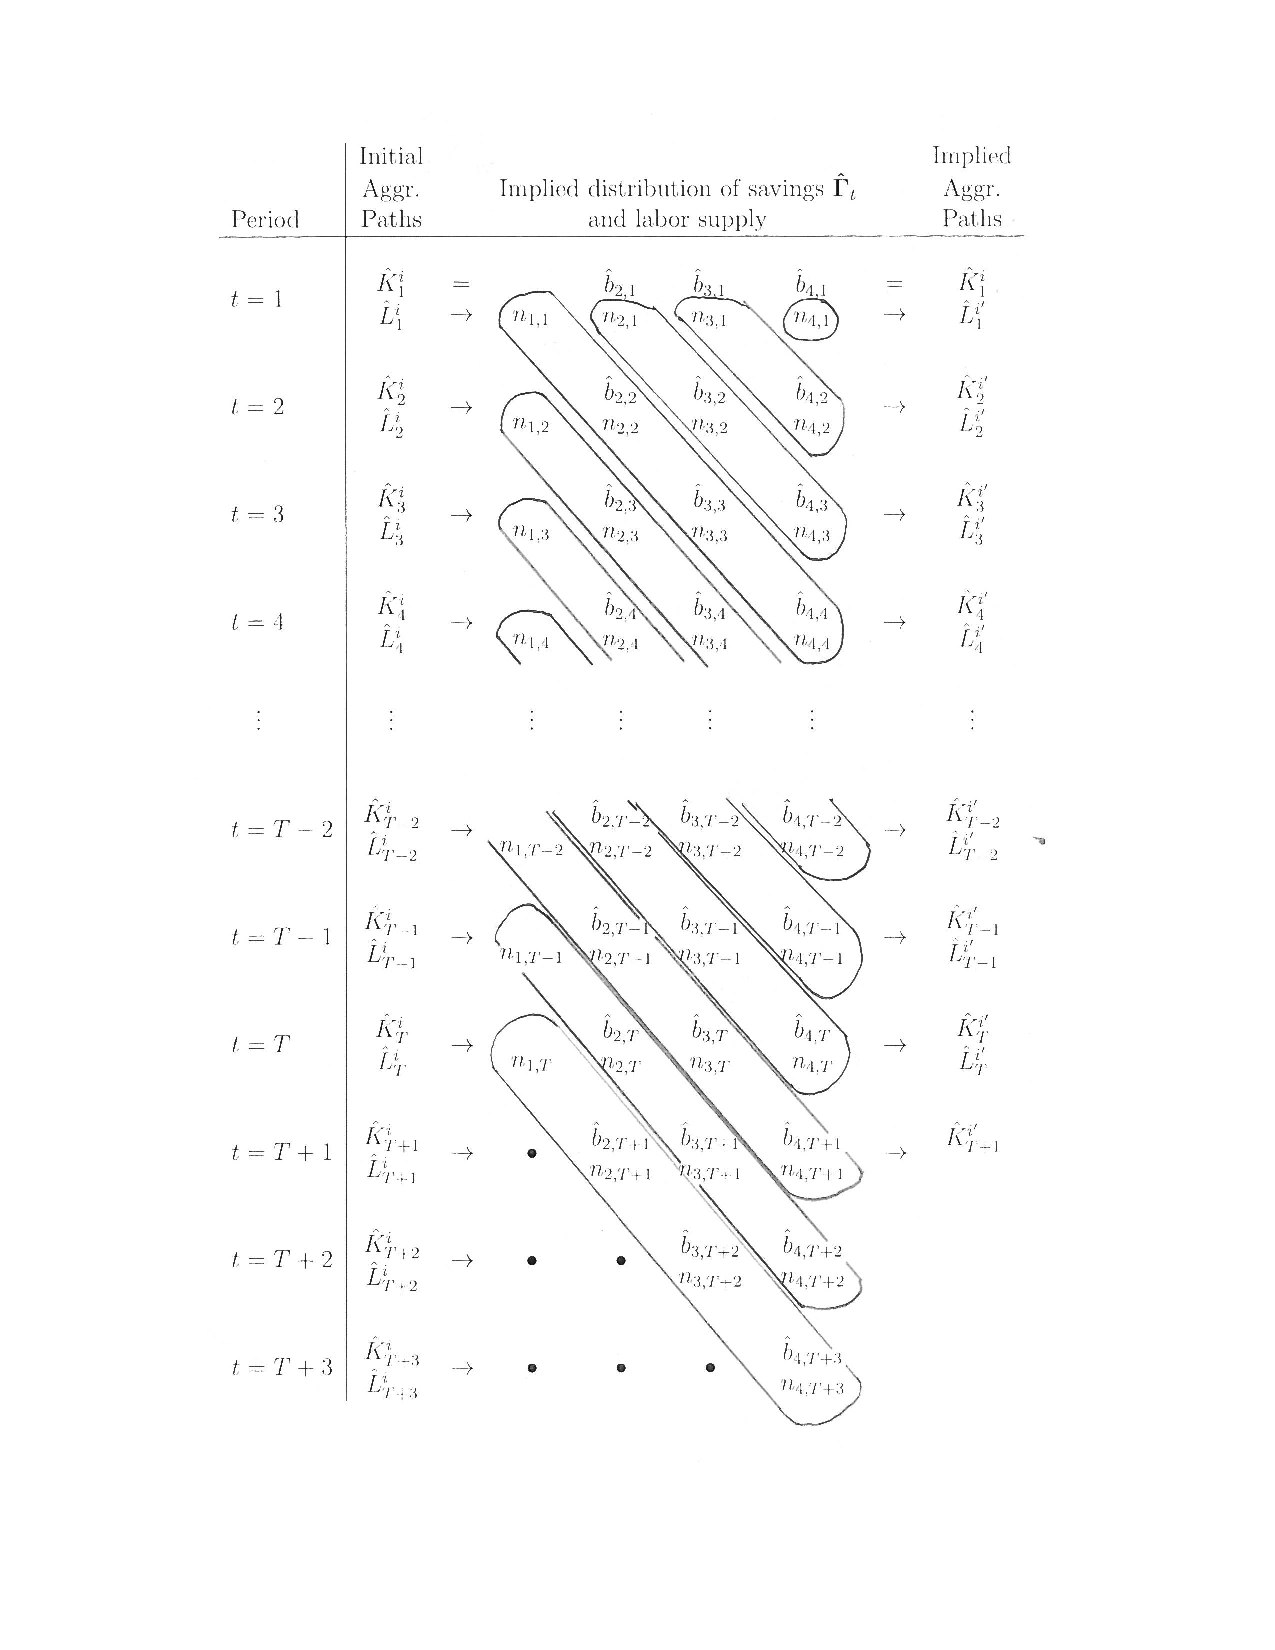
\includegraphics{images/TPIdiag.pdf}}}
  \end{figure}


  % THIS IS THE CODE FOR THE TABLE UNDERLYING THE FIGURE ABOVE
  % \begin{tabular}{>{\footnotesize}l| >{\footnotesize}c >{\footnotesize}c >{\footnotesize}c >{\footnotesize}c >{\footnotesize}c >{\footnotesize}c >{\footnotesize}c >{\footnotesize}c >{\footnotesize}c}
  %          & Initial & & & & & & & & Implied \\
  %          & Aggr. & & \multicolumn{5}{c}{Implied distribution of savings $\bm{\hat{\Gamma}}_t$} & & Aggr. \\
  %   Period & Paths    & & \multicolumn{5}{c}{and labor supply}   & & Paths    \\
  %   \hline
  %   & & & & & & & & & \\
  %   $t=1$ & $\begin{matrix}\hat{K}_1^i, \: \hat{BQ}_{j,1}^i \\ \hat{L}_1^i\end{matrix}$ & $\begin{matrix}= \\ \rightarrow\end{matrix}$ & $\begin{matrix}\: \\ n_{1,1}\end{matrix}$ & $\begin{matrix}\hat{b}_{2,1} \\ n_{2,1}\end{matrix}$ & $\begin{matrix}\hat{b}_{3,1} \\ n_{3,1}\end{matrix}$ & $\begin{matrix}\hat{b}_{4,1} \\ n_{4,1}\end{matrix}$ & $\begin{matrix}\hat{bq}_{5,1} \\ \,\end{matrix}$ & $\begin{matrix}= \\ \rightarrow\end{matrix}$ & $\begin{matrix}\hat{K}_1^i, \: \hat{BQ}_{j,1}^{i'} \\ \hat{L}^{i'}_1\end{matrix}$ \\[10mm]
  %   $t=2$ & $\begin{matrix}\hat{K}_2^i, \: \hat{BQ}_{j,2}^i \\ \hat{L}^i_2\end{matrix}$ & $\rightarrow$ & $\begin{matrix}\: \\ n_{1,2}\end{matrix}$ & $\begin{matrix}\hat{b}_{2,2} \\ n_{2,2}\end{matrix}$ & $\begin{matrix}\hat{b}_{3,2} \\ n_{3,2}\end{matrix}$ & $\begin{matrix}\hat{b}_{4,2} \\ n_{4,2}\end{matrix}$ & $\begin{matrix}\hat{bq}_{5,2} \\ \,\end{matrix}$ & $\rightarrow$ & $\begin{matrix}\hat{K}_2^{i'}, \: \hat{BQ}_{j,2}^{i'} \\ \hat{L}^{i'}_2\end{matrix}$ \\[10mm]
  %   $t=3$ & $\begin{matrix}\hat{K}_3^i, \: \hat{BQ}_{j,3}^i \\ \hat{L}^i_3\end{matrix}$ & $\rightarrow$ & $\begin{matrix}\: \\ n_{1,3}\end{matrix}$ & $\begin{matrix}\hat{b}_{2,3} \\ n_{2,3}\end{matrix}$ & $\begin{matrix}\hat{b}_{3,3} \\ n_{3,3}\end{matrix}$ & $\begin{matrix}\hat{b}_{4,3} \\ n_{4,3}\end{matrix}$ & $\begin{matrix}\hat{bq}_{5,3} \\ \,\end{matrix}$ & $\rightarrow$ & $\begin{matrix}\hat{K}_3^{i'}, \: \hat{BQ}_{j,3}^{i'} \\ \hat{L}^{i'}_3\end{matrix}$ \\[10mm]
  %   $t=4$ & $\begin{matrix}\hat{K}_4^i, \: \hat{BQ}_{j,4}^i \\ \hat{L}^i_4\end{matrix}$ & $\rightarrow$ & $\begin{matrix}\: \\ n_{1,4}\end{matrix}$ & $\begin{matrix}\hat{b}_{2,4} \\ n_{2,4}\end{matrix}$ & $\begin{matrix}\hat{b}_{3,4} \\ n_{3,4}\end{matrix}$ & $\begin{matrix}\hat{b}_{4,4} \\ n_{4,4}\end{matrix}$ & $\begin{matrix}\hat{bq}_{5,4} \\ \,\end{matrix}$ & $\rightarrow$ & $\begin{matrix}\hat{K}_4^{i'}, \: \hat{BQ}_{j,4}^{i'} \\ \hat{L}^{i'}_4\end{matrix}$ \\[10mm]
  %   $\quad\vdots$ & $\vdots$ & & $\vdots$ & $\vdots$ & $\vdots$ & $\vdots$ & $\vdots$ & & $\vdots$ \\[10mm]
  %   $t=T-2$ & $\begin{matrix}\hat{K}_{T-2}^i, \: \hat{BQ}_{j,T-2}^i \\ \hat{L}^i_{T-2}\end{matrix}$ & $\rightarrow$ & $\begin{matrix}\: \\ n_{1,T-2}\end{matrix}$ & $\begin{matrix}\hat{b}_{2,T-2} \\ n_{2,T-2}\end{matrix}$ & $\begin{matrix}\hat{b}_{3,T-2} \\ n_{3,T-2}\end{matrix}$ & $\begin{matrix}\hat{b}_{4,T-2} \\ n_{4,T-2}\end{matrix}$ & $\begin{matrix}\hat{bq}_{5,T-2} \\ \,\end{matrix}$ & $\rightarrow$ & $\begin{matrix}\hat{K}_{T-2}^{i'}, \: \hat{BQ}_{j,T-2}^{i'} \\ \hat{L}^{i'}_{T-2}\end{matrix}$ \\[10mm]
  %   $t=T-1$ & $\begin{matrix}\hat{K}_{T-1}^i, \: \hat{BQ}_{j,T-1}^i \\ \hat{L}^i_{T-1}\end{matrix}$ & $\rightarrow$ & $\begin{matrix}\: \\ n_{1,T-1}\end{matrix}$ & $\begin{matrix}\hat{b}_{2,T-1} \\ n_{2,T-1}\end{matrix}$ & $\begin{matrix}\hat{b}_{3,T-1} \\ n_{3,T-1}\end{matrix}$ & $\begin{matrix}\hat{b}_{4,T-1} \\ n_{4,T-1}\end{matrix}$ & $\begin{matrix}\hat{bq}_{5,T-1} \\ \,\end{matrix}$ & $\rightarrow$ & $\begin{matrix}\hat{K}_{T-1}^{i'}, \: \hat{BQ}_{j,T-1}^{i'} \\ \hat{L}^{i'}_{T-1}\end{matrix}$ \\[10mm]
  %   $t=T$ & $\begin{matrix}\hat{K}_{T}^i, \: \hat{BQ}_{j,T}^i \\ \hat{L}^i_{T}\end{matrix}$ & $\rightarrow$ & $\begin{matrix}\: \\ n_{1,T}\end{matrix}$ & $\begin{matrix}\hat{b}_{2,T} \\ n_{2,T}\end{matrix}$ & $\begin{matrix}\hat{b}_{3,T} \\ n_{3,T}\end{matrix}$ & $\begin{matrix}\hat{b}_{4,T} \\ n_{4,T}\end{matrix}$ & $\begin{matrix}\hat{bq}_{5,T} \\ \,\end{matrix}$ & $\rightarrow$ & $\begin{matrix}\hat{K}_{T}^{i'}, \: \hat{BQ}_{j,T}^{i'} \\ \hat{L}^{i'}_{T}\end{matrix}$ \\[10mm]
  %   $t=T+1$ & $\begin{matrix}\hat{K}_{T+1}^i, \: \hat{BQ}_{j,T+1}^i \\ \hat{L}^i_{T+1}\end{matrix}$ & $\rightarrow$ & $\bullet$ & $\begin{matrix}\hat{b}_{2,T+1} \\ n_{2,T+1}\end{matrix}$ & $\begin{matrix}\hat{b}_{3,T+1} \\ n_{3,T+1}\end{matrix}$ & $\begin{matrix}\hat{b}_{4,T+1} \\ n_{4,T+1}\end{matrix}$ & $\begin{matrix}\hat{bq}_{5,T+1} \\ \,\end{matrix}$ & $\rightarrow$ & $\begin{matrix}\hat{K}_{T+1}^{i'}, \: \hat{BQ}_{j,T+1}^{i'} \\ \:\end{matrix}$ \\[10mm]
  %   $t=T+2$ & $\begin{matrix}\hat{K}_{T+2}^i, \: \hat{BQ}_{j,T+2}^i \\ \hat{L}^i_{T+2}\end{matrix}$ & $\rightarrow$ & $\bullet$ & $\bullet$ & $\begin{matrix}\hat{b}_{3,T+2} \\ n_{3,T+2}\end{matrix}$ & $\begin{matrix}\hat{b}_{4,T+2} \\ n_{4,T+2}\end{matrix}$ & $\begin{matrix}\hat{bq}_{5,T+2} \\ \,\end{matrix}$ & & \\[10mm]
  %   $t=T+3$ & $\begin{matrix}\hat{K}_{T+3}^i, \: \hat{BQ}_{j,T+3}^i \\ \hat{L}^i_{T+3}\end{matrix}$ & $\rightarrow$ & $\bullet$ & $\bullet$ & $\bullet$ & $\begin{matrix}\hat{b}_{4,T+3} \\ n_{4,T+3}\end{matrix}$ & $\begin{matrix}\hat{bq}_{5,T+3} \\ \,\end{matrix}$ & & \\[10mm]
  %   $t=T+4$ & $\begin{matrix}\hat{K}_{T+4}^i, \: \hat{BQ}_{j,T+4}^i \\ \hat{L}^i_{T+4}\end{matrix}$ & $\rightarrow$ & $\bullet$ & $\bullet$ & $\bullet$ & $\bullet$ & $\begin{matrix}\hat{bq}_{5,T+4} \\ \,\end{matrix}$ & & \\
  % \end{tabular}
  % \clearpage

  Once the set of lifetime saving and labor supply decisions has been computed for all individuals alive in $1\leq t\leq T$, we use the household decisions to compute a new implied time path of the aggregate capital stock and aggregate labor. The implied paths of the aggregate capital stock $\bm{\hat{K}}^{i'}=\{\hat{K}_1^i,\hat{K}_2^{i'},...\hat{K}_T^{i'}\}$, aggregate labor $\bm{\hat{L}}^{i'}=\{\hat{L}_1^i,\hat{L}_2^{i'},...\hat{L}_T^{i'}\}$, and total bequests received $\bm{\hat{BQ}}_j^{i'}=\{\hat{BQ}_{j,1}^i,\hat{BQ}_{j,2}^{i'},...\hat{BQ}_{j,T}^{i'}\}$ in general do not equal the initial guessed paths $\bm{\hat{K}}^{i}=\{\hat{K}_1^i,\hat{K}_2^{i},...\hat{K}_T^{i}\}$, $\bm{\hat{L}}^{i}=\{\hat{L}_1^i,\hat{L}_2^{i},...\hat{L}_T^{i}\}$, and $\bm{\hat{BQ}}_j^{i}=\{\hat{BQ}_{j,1}^i,\hat{BQ}_{j,2}^{i},...\hat{BQ}_{j,T}^{i}\}$ used to compute the household savings and labor supply decisions $\bm{\hat{K}}^{i'}\neq\bm{\hat{K}}^i$, $\bm{\hat{L}}^{i'}\neq\bm{\hat{L}}^i$, and $\bm{\hat{BQ}}_j^{i'}\neq\bm{\hat{BQ}}_j^i$.

  Let $\norm{\:\cdot\:}$ be a norm on the space of time paths of the aggregate capital stock $\bm{\hat{K}}\in\mathcal{K}\subset\mathbb{R}_{++}^T$, aggregate labor supply $\bm{\hat{L}}\in\mathcal{L}\subset\mathbb{R}_{++}^T$, and $J$ paths of total bequests received $\bm{\hat{BQ}}_j\in\mathcal{B}\subset\mathbb{R}_{++}^T$. Then the fixed point necessary for the equilibrium transition path from Definition \ref{DefEquilNonSS} has been found when the distance between these $J+2$ paths is arbitrarily close to zero.
  \begin{equation}\label{EqTPIconverge}
    \norm{\Bigl[\bm{\hat{K}}^{i'}, \bm{\hat{L}}^{i'},\bigl\{\bm{\hat{BQ}}_j^{i'}\bigr\}_{j=1}^J\Bigr] - \Bigl[\bm{\hat{K}}^{i},\bm{\hat{L}}^{i},\bigl\{\bm{\hat{BQ}}_j^{i}\bigr\}_{j=1}^J\Bigr]} \leq \ve \quad\text{for}\quad \ve>0
  \end{equation}
  If the fixed point has not been found $\norm{\Bigl[\bm{\hat{K}}^{i'}, \bm{\hat{L}}^{i'},\bigl\{\bm{\hat{BQ}}_j^{i'}\bigr\}_{j=1}^J\Bigr] - \Bigl[\bm{\hat{K}}^{i},\bm{\hat{L}}^{i},\bigl\{\bm{\hat{BQ}}_j^{i}\bigr\}_{j=1}^J\Bigr]} > \ve$, then new transition paths for the aggregate capital stock and aggregate labor are generated as a convex combination of $\Bigl[\bm{\hat{K}}^{i'},\bm{\hat{L}}^{i'},\bigl\{\bm{\hat{BQ}}_j^{i'}\bigr\}_{j=1}^J\Bigr]$ and $\Bigl[\bm{\hat{K}}^{i},\bm{\hat{L}}^{i},\bigl\{\bm{\hat{BQ}}_j^{i}\bigr\}_{j=1}^J\Bigr]$.
  \begin{equation}\label{EqTPInewpath}
    \begin{split}
      \bm{\hat{K}}^{i+1} &= \nu\bm{\hat{K}}^{i'} + (1-\nu)\bm{\hat{K}}^{i} \\
      \bm{\hat{L}}^{i+1} &= \nu\bm{\hat{L}}^{i'} + (1-\nu)\bm{\hat{L}}^{i} \\
      \bm{\hat{BQ}}_1^{i+1} &= \nu\bm{\hat{BQ}}_1^{i'} + (1-\nu)\bm{\hat{BQ}}_1^{i} \\
      &\vdots \\
      \bm{\hat{BQ}}_J^{i+1} &= \nu\bm{\hat{BQ}}_J^{i'} + (1-\nu)\bm{\hat{BQ}}_J^{i}
    \end{split} \quad\quad\text{for}\quad \nu\in(0,1]
  \end{equation}
  This process is repeated until the initial transition paths for the aggregate capital stock, aggregate labor, and total bequests received are consistent with the transition paths implied by those beliefs and household and firm optimization.

  In essence, the TPI method iterates on individual beliefs about the time path of prices represented by a time paths for the aggregate capital stock $\bm{\hat{K}}^i$, aggregate labor $\bm{\hat{L}}^i$, and total bequests received $\bm{\hat{BQ}}_j^i$ until a fixed point in beliefs is found that are consistent with the transition paths implied by optimization based on those beliefs.

  The following are the steps for computing a stationary non-steady-state equilibrium time path for the economy.
  \begin{enumerate}
    \item Input all initial parameters. See Table \ref{TabExogVars}.
      \begin{enumerate}
        \item The value for $T$ at which the non-steady-state transition path should have converged to the steady state should be at least as large as the number of periods it takes the population to reach its steady state $\bm{\bar{\omega}}$ as described in Appendix \ref{AppPopGrowth}.
      \end{enumerate}

    \item Choose an initial distribution of savings and intended bequests $\bm{\hat{\Gamma}}_1$ and then calculat the initial state of the stationarized aggregate capital stock $\hat{K}_1$ and total bequests received $\hat{BQ}_{j,1}$ consistent with $\bm{\hat{\Gamma}}_1$ according to \eqref{EqMktClrCapStat} and \eqref{EqTotBeqStat1}.
      \begin{enumerate}
        \item Note that you must have the population weights from the previous period $\hat{\omega}_{s,0}$ and the growth rate between period 0 and period 1 $\tilde{g}_{n,1}$to calculate $\hat{BQ}_{j,1}$.
      \end{enumerate}
    \item Conjecture transition paths for the stationarized aggregate capital stock $\bm{\hat{K}}^1=\{\hat{K}^1_t\}_{t=1}^\infty$, stationarized aggregate labor $\bm{\hat{L}}^1=\{\hat{L}^1_t\}_{t=1}^\infty$, and total bequests received $\bm{\hat{BQ}}_j^1=\{\hat{BQ}^{1}_{j,t}\}_{t=1}^\infty$ where the only requirements are that $\hat{K}^i_1$ and $\hat{BQ}^i_{j,1}$ are functions of the initial distribution of savings $\bm{\hat{\Gamma}}_1$ for all $i$ is your initial state and that $\hat{K}^i_t=\bar{K}$, $\hat{L}^i_t=\bar{L}$, and $\hat{BQ}^i_{j,t}= \bar{BQ}_j$ for all $t\geq T$. The conjectured transition paths of the aggregate capital stock $\bm{\hat{K}}^i$ and aggregate labor $\bm{\hat{L}}^i$ imply specific transition paths for the real wage $\bm{\hat{w}}^i=\{\hat{w}^i_t\}_{t=1}^\infty$ and the real interest rate $\bm{r}^i=\{r^i_t\}_{t=1}^\infty$ through expressions \eqref{EqFOCwageStat} and \eqref{EqFOCrate}.
      \begin{enumerate}
        \item An intuitive choice for the time path of aggregate labor is the steady-state in every period $\hat{L}^1_t = \bar{L}$ for all $t$.
      \end{enumerate}
    \item With the conjectured transition paths $\bm{\hat{w}}^i$, $\bm{r}^i$, and $\bm{\hat{BQ}}_j^i$ one can solve for the lifetime policy functions of each household alive at time $1\leq t\leq T$ using the systems of Euler equations of the form \eqref{EqEulerLabStat}, \eqref{EqEulerSavStat}, and \eqref{EqEulerBeqStat} and following the diagram in Figure \ref{FigTPIdiag}.
      \begin{enumerate}
        \item Make sure that the individual borrowing constraints \eqref{EqSavMin} are satisfied for each individual in every period.
        \item Increase any individual savings to the minimum $\tilde{b}_{j,s,t}$ if the borrowing constraint is not satisfied.
      \end{enumerate}
    \item Use the implied distribution of savings and labor supply in each period (each row of $\hat{b}_{j,s,t}$ and $n_{j,s,t}$ in Figure \ref{FigTPIdiag}) to compute the new implied time paths for the aggregate capital stock $\bm{\hat{K}}^{i'} = \{\hat{K}_1^i,\hat{K}_2^{i'},...\hat{K}_T^{i'}\}$, aggregate labor supply $\bm{\hat{L}}^{i'} = \{\hat{L}_1^i,\hat{L}_2^{i'},...\hat{L}_T^{i'}\}$, and total bequests received $\bm{\hat{BQ}}_j^{i'} = \{\hat{BQ}_{j,1}^i,\hat{BQ}_{j,2}^{i'},...\hat{BQ}_{j,T}^{i'}\}$.
      \begin{enumerate}
        \item Make sure that the aggregate borrowing constraint \eqref{EqAggrCapConstr} and total bequests constraint $\hat{BQ}_{j,t}\geq 0$ are satisfied in each period $t$.
        \item If the aggregate borrowing constraint is not satisfied, increase every individual's savings by the fraction that makes the aggregate capital stock slightly greater than zero.
      \end{enumerate}
    \item Check the distance between the two sets time paths.
      \begin{equation*}
        \norm{\Bigl[\bm{\hat{K}}^{i'}, \bm{\hat{L}}^{i'},\bigl\{\bm{\hat{BQ}}_j^{i'}\bigr\}_{j=1}^J\Bigr] - \Bigl[\bm{\hat{K}}^{i},\bm{\hat{L}}^{i},\bigl\{\bm{\hat{BQ}}_j^{i}\bigr\}_{j=1}^J\Bigr]}
      \end{equation*}
      \begin{enumerate}
        \item If the distance between the initial time paths and the implied time paths is less-than-or-equal-to some convergence criterion $\ve>0$, then the fixed point has been achieved and the equilibrium time path has been found \eqref{EqTPIconverge}.
        \item If the distance between the initial time paths and the implied time paths is greater than some convergence criterion $\norm{\cdot}>\ve$, then update the guess for the time paths according to \eqref{EqTPInewpath} and repeat steps (4) through (6) until a fixed point is reached.
      \end{enumerate}
  \end{enumerate}

  \clearpage


\newpage
\bibliography{DynScoreMacro_popdist}



\newpage
\renewcommand{\theequation}{T.\arabic{section}.\arabic{equation}}
                                                 % redefine the command that creates the section number
\renewcommand{\thesection}{T-\arabic{section}}   % redefine the command that creates the equation number
\setcounter{equation}{0}                         % reset counter
\setcounter{section}{0}                          % reset section number
\section*{TECHNICAL APPENDIX}


\section{Comments and Notes}\label{TAppComments}

  \noindent Structures to add to the model and order
  \begin{enumerate}
    \item Add household tax structures
    \item Add firm structures
    \item Add small open economy feature
  \end{enumerate}


\end{document}
